\documentclass[12pt,a4paper]{article}

% =========================================================================
% FORMATAÇÃO ABNT (NBR 14724 / NBR 6024 / NBR 6027)
% =========================================================================

% --- Margens ABNT (3 cm superior e esquerda; 2 cm inferior e direita) ---
\usepackage[
  a4paper,
  left=3cm,
  top=3cm,
  right=2cm,
  bottom=2cm,
  headheight=15pt,
  headsep=1cm
]{geometry}

% --- Idioma, codificação e tipografia (Times New Roman - ABNT NBR 14724) ---
\usepackage[T1]{fontenc}
\usepackage[utf8]{inputenc}
\usepackage[brazil]{babel}
\usepackage{amsmath}
\usepackage{newtxtext,newtxmath}
\usepackage{microtype}
\usepackage[htt]{hyphenat} % permite quebra de linha em identificadores \texttt

% --- Espaçamento e parágrafo ABNT ---
\usepackage{setspace}
\onehalfspacing                    % 1,5 entre linhas para o texto
\usepackage{indentfirst}           % recuo no primeiro parágrafo
\setlength{\parindent}{1.25cm}     % recuo padrão ABNT
\setlength{\parskip}{0pt}
\setlength{\emergencystretch}{2em} % evita linhas muito longas (overfull hbox)

% --- Tabelas e alinhamentos ---
\usepackage{array}
\usepackage{tabularx}
\usepackage{xltabular}
\usepackage{needspace}
\usepackage{enumitem}
\usepackage{booktabs}
\usepackage{etoolbox}

% --- Figuras, quadros e imagens ---
\usepackage{graphicx}
\graphicspath{{../assets/}{assets/}}
\usepackage{float}
\usepackage{pdflscape}

% --- Cabeçalhos e paginação ABNT (NBR 14724 item 5.3) ---
% Numeração arábica visível no canto superior direito (2 cm do topo, 2 cm da borda direita).
% Páginas pré-textuais contadas sem numeração aparente.
\usepackage{fancyhdr}
\pagestyle{empty}
\fancyhf{}
\fancyhead[R]{\small\thepage}
\renewcommand{\headrulewidth}{0pt}

% --- Formatação do Sumário (NBR 6027) ---
\usepackage{tocloft}
\renewcommand{\cftsecleader}{\cftdotfill{\cftdotsep}}
\renewcommand{\cftsecfont}{\bfseries}
\renewcommand{\cftsecpagefont}{\bfseries}
\setlength{\cftbeforesecskip}{0.4em}

% --- Formatação dos títulos de seções (NBR 6024) ---
\usepackage{titlesec}
% 1 SEÇÃO PRIMÁRIA (caixa alta, negrito)
\titleformat{\section}
  {\normalfont\normalsize\bfseries\MakeUppercase}{\thesection}{1em}{}
% 1.1 Seção secundária (negrito)
\titleformat{\subsection}
  {\normalfont\normalsize\bfseries}{\thesubsection}{1em}{}
% 1.1.1 Seção terciária (negrito)
\titleformat{\subsubsection}
  {\normalfont\normalsize\bfseries}{\thesubsubsection}{1em}{}
% 1.1.1.1 Seção quaternária (itálico)
\titleformat{\paragraph}
  {\normalfont\normalsize\itshape}{\theparagraph}{1em}{}

\titlespacing*{\section}{0pt}{2ex plus 0.5ex minus 0.2ex}{1.5ex plus 0.5ex minus 0.2ex}
\titlespacing*{\subsection}{0pt}{1.8ex plus 0.5ex minus 0.2ex}{1.2ex plus 0.5ex minus 0.2ex}
\titlespacing*{\subsubsection}{0pt}{1.5ex plus 0.5ex minus 0.2ex}{1.0ex plus 0.5ex minus 0.2ex}

% --- Legendas e fontes (NBR 14724 / IBGE) ---
\usepackage{caption}
\captionsetup{
  font=small,
  labelfont=bf,
  justification=centering,
  singlelinecheck=false,
  skip=6pt
}
\captionsetup[figure]{name=Figura, labelsep=colon}
\captionsetup[table]{name=Quadro, labelsep=colon}

% "Fonte:" abaixo de figuras e quadros
\newcommand{\fonte}[1]{%
  \par\vspace{2pt}%
  {\footnotesize\centering\textbf{Fonte:} #1\par}%
}

% Espaçamento simples dentro de figuras e quadros (exigência ABNT)
\AtBeginEnvironment{figure}{\singlespace}
\AtBeginEnvironment{table}{\singlespace}
\AtBeginEnvironment{xltabular}{\singlespace}

% --- Códigos-fonte (PlantUML) ---
\usepackage[table]{xcolor}
\definecolor{ghlight}{RGB}{225,229,233}
\definecolor{ghbg}{RGB}{246,248,250}
\usepackage{listings}
% pdfLaTeX: converte UTF-8 -> latin1 nos listings (garante acentuação correta)
\ifdefined\pdftexversion
  \usepackage{listingsutf8}
\fi
\definecolor{codgray}{gray}{0.45}
\lstset{
  basicstyle=\ttfamily\footnotesize,
  breaklines=true,
  columns=fullflexible,
  keepspaces=true,
  showstringspaces=false,
  frame=single,
  framexleftmargin=4pt,
  tabsize=2,
  numbers=left,
  numberstyle=\tiny\color{codgray},
  numbersep=8pt,
  xleftmargin=20pt,
  captionpos=b
}
% pdfLaTeX precisa decodificar UTF-8 explicitamente nos listings
\ifdefined\pdftexversion
  \lstset{inputencoding=utf8/latin1, extendedchars=true}
\fi

% --- Listas compactas ---
\providecommand{\tightlist}{%
  \setlength{\itemsep}{0pt}\setlength{\parskip}{0pt}}

% --- Links e marcadores ---
\usepackage[hidelinks]{hyperref}
\usepackage{bookmark}
\IfFileExists{xurl.sty}{\usepackage{xurl}}{}
\urlstyle{same}


\begin{document}

% --- CAPA ---
\begin{titlepage}
  \thispagestyle{empty}
  \begin{center}
    \textbf{\large UNIVERSIDADE FEDERAL DE GOIÁS}\\[0.2cm]
    \textbf{\large INSTITUTO DE INFORMÁTICA}\\[0.2cm]
    \textbf{\large BACHARELADO EM ENGENHARIA DE SOFTWARE}\\[0.2cm]
    \textbf{\large DISCIPLINA: MODELAGEM DE SOFTWARE}

    \vspace{3.2cm}
    {\large
    \begin{tabular}{@{}l@{\hspace{2.5em}}l@{}}
      \textbf{Nome} & \textbf{Matrícula}\\[0.2cm]
      Carlos Eduardo Freire da Silva & 202602990\\
      Gabriel Henrique Lourenço Dias & 202602992\\
      Kayque Vicente Silva & 202605511\\
      Luiz Pedro Pereira Mendes Saraiva & 202605512\\
      Yury Nogueira de Oliveira Silva & 202600700\\
    \end{tabular}\par}

    \vspace{3.5cm}
    \textbf{\Large SITE DE LOJA DE ELETRÔNICOS (E-COMMERCE)}\\[0.4cm]
    \textbf{\large Modelagem de Software: APS2}\par

    \vfill
    \textbf{GOIÂNIA}\\[0.2cm]
    \textbf{2026}
  \end{center}
\end{titlepage}

% --- FOLHA DE ROSTO ---
\thispagestyle{empty}
\begin{center}
  {\large
  Carlos Eduardo Freire da Silva\\
  Gabriel Henrique Lourenço Dias\\
  Kayque Vicente Silva\\
  Luiz Pedro Pereira Mendes Saraiva\\
  Yury Nogueira de Oliveira Silva\par}

  \vspace{4.0cm}
  \textbf{\Large SITE DE LOJA DE ELETRÔNICOS (E-COMMERCE)}\\[0.4cm]
  \textbf{\large Modelagem de Software: APS2}\par
\end{center}

\vspace{2.5cm}
\begin{flushright}
  \begin{minipage}{0.52\textwidth}
    \begin{singlespace}
      {\small Trabalho acadêmico apresentado à disciplina de Modelagem
      de Software do curso de Bacharelado em Engenharia de Software da
      Universidade Federal de Goiás (UFG), como requisito parcial de
      avaliação referente à Atividade Prática Supervisionada (APS2).\\[0.4cm]
      \textbf{Professor Orientador:} Prof. Me. Diogo Oliveira Santos}
    \end{singlespace}
  \end{minipage}
\end{flushright}

\vfill
\begin{center}
  \textbf{GOIÂNIA}\\[0.2cm]
  \textbf{2026}
\end{center}
\newpage

% --- SUMÁRIO ---
\thispagestyle{empty}
\renewcommand{\contentsname}{SUMÁRIO}
\pdfbookmark[0]{\contentsname}{toc}
\tableofcontents
\newpage

\pagestyle{fancy}
\thispagestyle{fancy}

% =========================================================================
\section{Visão Geral do Sistema}\label{sec:visao}

\subsection{Descrição e Contexto}

O tema escolhido é o \textbf{Site de Loja de Eletrônicos (e-commerce)}, uma
loja virtual de produtos eletrônicos de consumo, como smartphones, notebooks,
tablets, televisores, fones de ouvido e acessórios. O público são consumidores
finais, que compram pela internet e recebem o pedido em casa. Como esse tipo de
produto tem muitos modelos, marcas e faixas de preço, o cliente navega por um
catálogo com filtros por categoria, marca e preço, adiciona itens a um
carrinho e finaliza o pedido. O pagamento e o cálculo de frete são feitos por
serviços externos (um \textbf{gateway de pagamento} e um \textbf{serviço de
frete}), e o cliente é avisado por e-mail sobre o andamento do pedido. Do lado
da loja, uma \textbf{área administrativa} permite cadastrar produtos, controlar
o estoque, que é limitado e muda a cada venda, e acompanhar o status dos
pedidos.

Este trabalho apresenta os casos de uso em um único diagrama, descritos em
tabelas, e a arquitetura em diagramas de componentes, em dois níveis. Os
requisitos completos estão no Apêndice~\ref{sec:apendice} e os termos técnicos
são explicados no Apêndice~\ref{sec:termos}.

\subsection{Escopo}

\noindent\textbf{Dentro do escopo:}
\begin{itemize}
\tightlist
\item cadastro e autenticação de clientes e do administrador;
\item catálogo de produtos, com navegação, filtros e busca;
\item carrinho de compras;
\item finalização do pedido, com cálculo de frete e pagamento (cartão, Pix ou boleto);
\item consulta e cancelamento de pedidos pelo cliente;
\item área administrativa: produtos, estoque e status dos pedidos;
\item avisos por e-mail ao cliente.
\end{itemize}

\noindent\textbf{Fora do escopo:}
\begin{itemize}
\tightlist
\item cupons e promoções;
\item avaliações de produtos;
\item troca e devolução;
\item nota fiscal;
\item marketplace (vários vendedores) e aplicativo nativo.
\end{itemize}

\subsection{Premissas}\label{sec:premissas}

\begin{itemize}
\tightlist
\item O sistema é um \textbf{web app responsivo}.
\item Cadastro e autenticação foram acrescentados, pois finalizar pedido e
  acessar a área administrativa pressupõem identificação.
\item Há um \textbf{único perfil administrativo}.
\item As formas de pagamento são \textbf{cartão, Pix e boleto}, todas pelo
  gateway de pagamento.
\item O visitante pode montar o carrinho; a autenticação é exigida só na
  finalização do pedido.
\item O único canal de notificação é o \textbf{e-mail}.
\item Categorias e marcas são criadas pelo administrador ao cadastrar o produto.
\item O pedido aguardando pagamento é cancelado após um prazo, e o estoque reservado é devolvido.
\item Os produtos e as categorias citados são exemplos adotados pelo grupo; o
  catálogo real é cadastrado pelo administrador.
\end{itemize}

% =========================================================================
\section{Diagrama de Casos de Uso}\label{sec:uc}

Os casos de uso foram derivados dos requisitos do Apêndice~\ref{sec:apendice}. Os que um ator aciona diretamente são o CU\nobreakdash-01 a CU\nobreakdash-06 e o CU\nobreakdash-12. Os demais (CU\nobreakdash-07 a CU\nobreakdash-11 e CU\nobreakdash-13) são casos de apoio: partes reutilizadas ou opcionais dos primeiros, ligadas a eles por \texttt{<<include>>} ou \texttt{<<extend>>}. Este capítulo apresenta os atores, os relacionamentos e o diagrama, explica as decisões de modelagem e, por fim, especifica cada caso de uso em uma tabela.

\subsection{Atores}

\begin{itemize}
\tightlist
\item \textbf{Visitante} (principal): navega, filtra e busca produtos,
  sem autenticação.
\item \textbf{Cliente} (principal): visitante autenticado; finaliza e
  consulta pedidos. Herda do Visitante (generalização).
\item \textbf{Administrador} (principal): gerencia produtos, estoque e
  pedidos.
\item \textbf{Gateway de Pagamento} (secundário, sistema externo):
  autoriza e estorna pagamentos.
\item \textbf{Serviço de Frete} (secundário, sistema externo): calcula
  valor e prazo de entrega.
\item \textbf{Serviço de E-mail} (secundário, sistema externo): envia as
  mensagens de status do pedido.
\end{itemize}

\subsection{Relacionamentos}

\begin{itemize}
\setlength{\itemsep}{0.4em}
\item \textbf{Associação:} liga cada ator aos casos de uso em que ele participa.
\item \textbf{Generalização:} o Cliente herda do Visitante e pode fazer tudo o que o visitante faz.
\item \textbf{\texttt{<<include>>}:} o caso de uso de origem sempre executa o caso de destino. É um passo obrigatório e reutilizável.
\item \textbf{\texttt{<<extend>>}:} o caso de uso de origem acrescenta um fluxo opcional ao caso de destino, só quando uma condição acontece. A condição aparece em uma nota, ligada à seta por uma linha tracejada.
\end{itemize}

\subsection{Diagrama}

\begin{figure}[H]
\centering
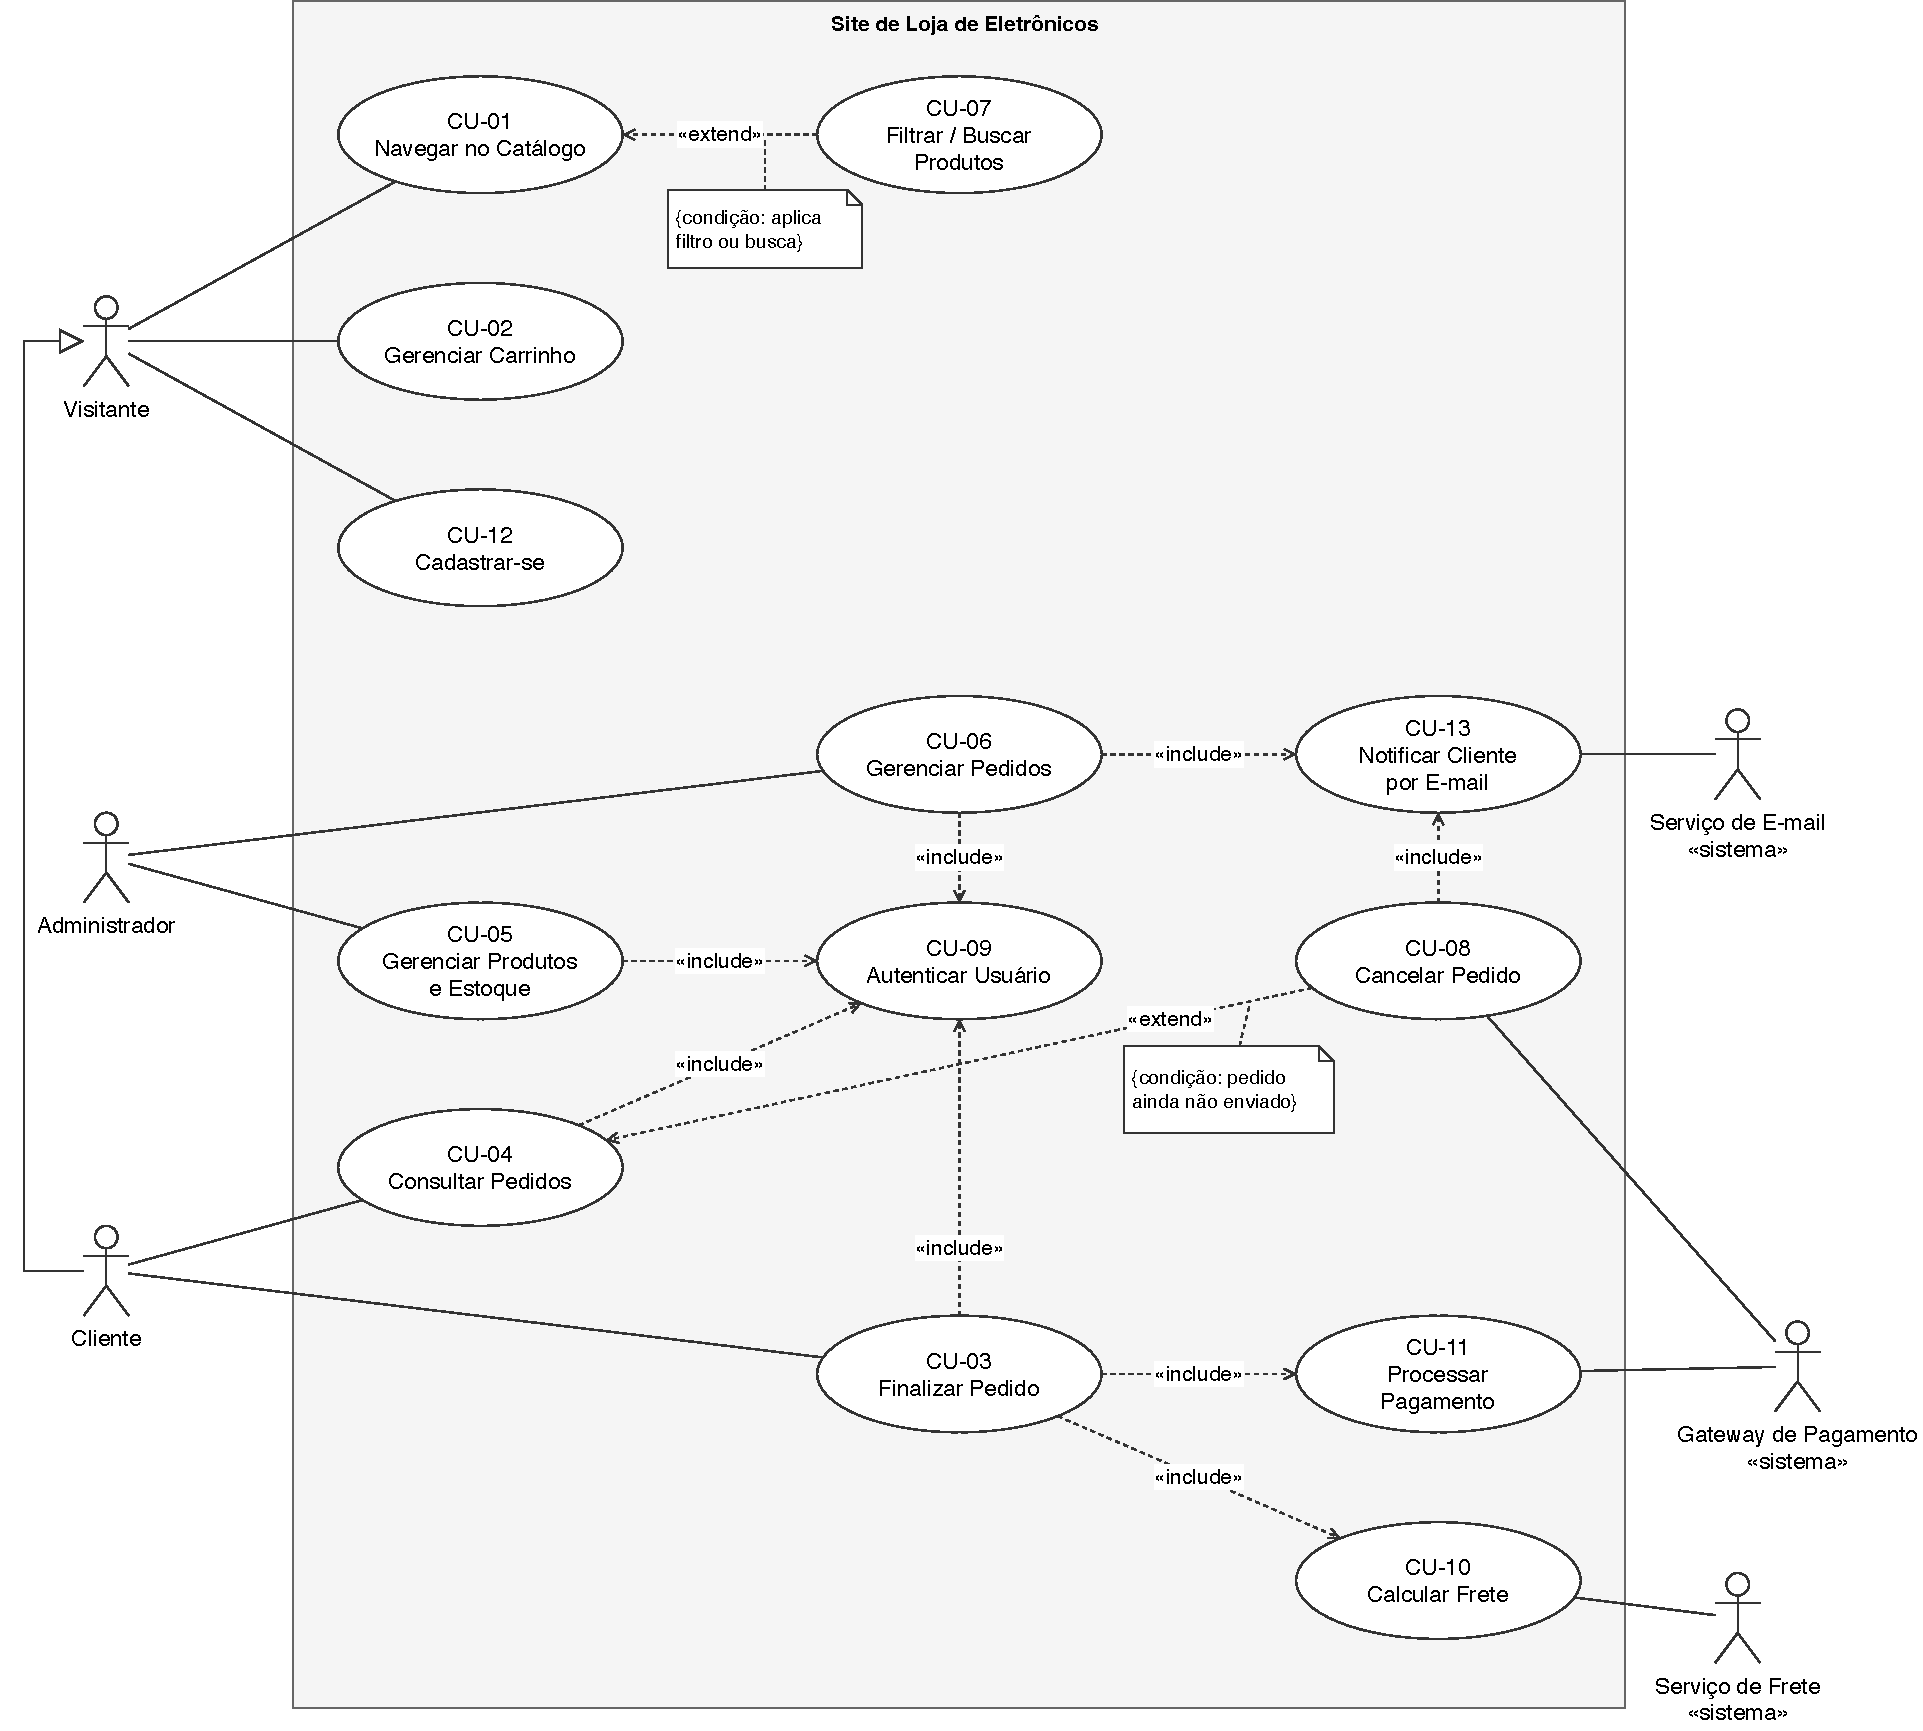
\includegraphics[width=\textwidth,height=0.72\textheight,keepaspectratio]{../assets/CU_CasosDeUso.pdf}
\caption{Diagrama de Casos de Uso do Site de Loja de Eletrônicos}
\fonte{elaborado pelos autores no draw.io (2026).}
\end{figure}

O quadro a seguir lista cada relacionamento \texttt{<<include>>} e \texttt{<<extend>>}, na direção da seta do diagrama acima.

{\arrayrulecolor{ghlight}\setlength{\arrayrulewidth}{0.3pt}\renewcommand{\arraystretch}{1.15}\rowcolors{2}{ghbg}{white}\small
\begin{xltabular}{\textwidth}{>{\raggedright\arraybackslash}p{2.4cm}|>{\raggedright\arraybackslash}p{3.7cm}|>{\raggedright\arraybackslash}p{3.7cm}|>{\raggedright\arraybackslash}X}
\rowcolor{white}\caption{Relacionamentos \texttt{<<include>>} e \texttt{<<extend>>} do diagrama}\\
\arrayrulecolor{black}\toprule\arrayrulecolor{ghlight}
\rowcolor{ghbg}\textbf{Tipo} & \textbf{Origem da seta} & \textbf{Destino da seta} & \textbf{Quando ocorre}\\ \arrayrulecolor{black}\midrule\arrayrulecolor{ghlight}
\endfirsthead
\arrayrulecolor{black}\toprule\arrayrulecolor{ghlight}
\rowcolor{ghbg}\textbf{Tipo} & \textbf{Origem da seta} & \textbf{Destino da seta} & \textbf{Quando ocorre}\\ \arrayrulecolor{black}\midrule\arrayrulecolor{ghlight}
\endhead
\endlastfoot
\texttt{<<include>>} & CU\nobreakdash-03 Finalizar Pedido & CU\nobreakdash-09 Autenticar Usuário & Só o cliente autenticado finaliza um pedido.\\ \hline
\texttt{<<include>>} & CU\nobreakdash-03 Finalizar Pedido & CU\nobreakdash-10 Calcular Frete & Sem o frete não há valor total do pedido.\\ \hline
\texttt{<<include>>} & CU\nobreakdash-03 Finalizar Pedido & CU\nobreakdash-11 Processar Pagamento & O pedido só avança com o pagamento.\\ \hline
\texttt{<<include>>} & CU\nobreakdash-04 Consultar Pedidos & CU\nobreakdash-09 Autenticar Usuário & Cada cliente só vê os próprios pedidos.\\ \hline
\texttt{<<include>>} & CU\nobreakdash-05 Gerenciar Produtos e Estoque & CU\nobreakdash-09 Autenticar Usuário & A área administrativa é restrita.\\ \hline
\texttt{<<include>>} & CU\nobreakdash-06 Gerenciar Pedidos & CU\nobreakdash-09 Autenticar Usuário & A área administrativa é restrita.\\ \hline
\texttt{<<include>>} & CU\nobreakdash-06 Gerenciar Pedidos & CU\nobreakdash-13 Notificar Cliente por E-mail & O cliente é avisado a cada mudança de status.\\ \hline
\texttt{<<include>>} & CU\nobreakdash-08 Cancelar Pedido & CU\nobreakdash-13 Notificar Cliente por E-mail & O cliente é avisado do cancelamento.\\ \hline
\texttt{<<extend>>} & CU\nobreakdash-07 Filtrar / Buscar Produtos & CU\nobreakdash-01 Navegar no Catálogo & Quando o visitante aplica um filtro ou faz uma busca.\\ \hline
\texttt{<<extend>>} & CU\nobreakdash-08 Cancelar Pedido & CU\nobreakdash-04 Consultar Pedidos & Quando o cliente decide cancelar, e só se o pedido ainda não foi enviado.\\ \arrayrulecolor{black}\bottomrule
\end{xltabular}}

\subsection{Decisões de Modelagem}

\begin{itemize}
\setlength{\itemsep}{0.4em}
\item \textbf{Cliente herda de Visitante:} o visitante já navega e monta o carrinho sem conta; o cliente é o visitante autenticado e ganha o que exige identificação (finalizar e consultar pedidos). Assim os casos de navegação não se repetem para os dois.
\item \textbf{Autenticar Usuário é \texttt{<<include>>}:} é um passo obrigatório e igual para quem finaliza ou consulta pedidos e para o administrador, então fica em um caso só, reutilizado.
\item \textbf{Calcular Frete e Processar Pagamento são \texttt{<<include>>} de Finalizar Pedido:} o pedido não existe sem eles, e cada um envolve um sistema externo. Separá-los mostra quem participa de quê (Serviço de Frete e Gateway de Pagamento).
\item \textbf{Filtrar / Buscar e Cancelar são \texttt{<<extend>>}:} o fluxo se completa sem eles; só entram quando a condição acontece.
\item \textbf{Notificar Cliente por E-mail é um caso à parte:} dois casos disparam o aviso (CU\nobreakdash-06 e CU\nobreakdash-08), e assim o Serviço de E-mail aparece em um ponto só.
\item \textbf{Cadastrar-se é um caso próprio do Visitante:} é a forma de virar cliente, e não uma variação do login.
\end{itemize}

\Needspace{22\baselineskip}
\subsection{Especificação Textual dos Casos de Uso}

\Needspace{200pt}
\subsubsection{CU-01: Navegar no Catálogo}

{\arrayrulecolor{ghlight}\setlength{\arrayrulewidth}{0.3pt}\renewcommand{\arraystretch}{1.1}\small\rowcolors{2}{ghbg}{white}
\begin{xltabular}{\textwidth}{>{\raggedright\arraybackslash}p{3.4cm}|>{\raggedright\arraybackslash}X}
\rowcolor{white}\caption{Especificação do CU-01}\\
\arrayrulecolor{black}\toprule\arrayrulecolor{ghlight}
\rowcolor{ghbg}\textbf{Campo} & \textbf{Descrição}\\ \arrayrulecolor{black}\midrule\arrayrulecolor{ghlight}
\endfirsthead
\arrayrulecolor{black}\toprule\arrayrulecolor{ghlight}
\rowcolor{ghbg}\textbf{Campo} & \textbf{Descrição}\\ \arrayrulecolor{black}\midrule\arrayrulecolor{ghlight}
\endhead
\endlastfoot
Nome & CU\nobreakdash-01: Navegar no Catálogo\\ \hline
Atores envolvidos & \textbf{Visitante}.\\ \hline
Pré-condições & Nenhuma.\\ \hline
Fluxo principal & \begin{enumerate}[nosep,leftmargin=1.4em,label=\arabic*.,before=\vspace{-\baselineskip},after=\vspace{-0.4\baselineskip}]\item O \textbf{Visitante} acessa o catálogo. \item O sistema lista os produtos ativos da loja. \item O \textbf{Visitante} abre um produto. \item O sistema mostra os detalhes e a disponibilidade. \end{enumerate}\\ \hline
Fluxos alternativos ou de exceção & \begin{itemize}[nosep,leftmargin=2.2em,labelwidth=2.2em,labelsep=0pt,align=left,itemsep=4pt,before=\vspace{-\baselineskip},after=\vspace{-0.4\baselineskip}]\item[\textbf{A1}] No passo 2, se o \textbf{Visitante} aplica um filtro ou faz uma busca,\par então o sistema atualiza a lista (CU\nobreakdash-07). \item[\textbf{A2}] No passo 2, se nenhum produto atende ao filtro,\par então o sistema sugere limpar os filtros.\end{itemize}\\ \arrayrulecolor{black}\bottomrule
\end{xltabular}}

\Needspace{200pt}
\subsubsection{CU-02: Gerenciar Carrinho}

{\arrayrulecolor{ghlight}\setlength{\arrayrulewidth}{0.3pt}\renewcommand{\arraystretch}{1.1}\small\rowcolors{2}{ghbg}{white}
\begin{xltabular}{\textwidth}{>{\raggedright\arraybackslash}p{3.4cm}|>{\raggedright\arraybackslash}X}
\rowcolor{white}\caption{Especificação do CU-02}\\
\arrayrulecolor{black}\toprule\arrayrulecolor{ghlight}
\rowcolor{ghbg}\textbf{Campo} & \textbf{Descrição}\\ \arrayrulecolor{black}\midrule\arrayrulecolor{ghlight}
\endfirsthead
\arrayrulecolor{black}\toprule\arrayrulecolor{ghlight}
\rowcolor{ghbg}\textbf{Campo} & \textbf{Descrição}\\ \arrayrulecolor{black}\midrule\arrayrulecolor{ghlight}
\endhead
\endlastfoot
Nome & CU\nobreakdash-02: Gerenciar Carrinho\\ \hline
Atores envolvidos & \textbf{Visitante}; \textbf{Cliente}.\\ \hline
Pré-condições & Produto ativo e disponível.\\ \hline
Fluxo principal & \begin{enumerate}[nosep,leftmargin=1.4em,label=\arabic*.,before=\vspace{-\baselineskip},after=\vspace{-0.4\baselineskip}]\item O \textbf{Visitante} ou o \textbf{Cliente} adiciona um produto ao carrinho, informando a quantidade. \item O sistema confere a disponibilidade. \item O sistema atualiza o carrinho e o subtotal. \item O \textbf{Visitante} ou o \textbf{Cliente} altera quantidades ou remove itens. \item O \textbf{Visitante} ou o \textbf{Cliente} segue para a finalização do pedido (CU\nobreakdash-03) ou continua comprando. \end{enumerate}\\ \hline
Fluxos alternativos ou de exceção & \begin{itemize}[nosep,leftmargin=2.2em,labelwidth=2.2em,labelsep=0pt,align=left,itemsep=4pt,before=\vspace{-\baselineskip},after=\vspace{-0.4\baselineskip}]\item[\textbf{A1}] No passo 5, se o \textbf{Visitante} se autentica na finalização,\par então os itens do carrinho dele passam para a conta do \textbf{Cliente}. \item[\textbf{E1}] No passo 2, se a quantidade pedida é maior que o estoque,\par então o sistema limita ao disponível e avisa. \item[\textbf{E2}] No passo 3, se um item fica indisponível,\par então o sistema sinaliza no carrinho.\end{itemize}\\ \arrayrulecolor{black}\bottomrule
\end{xltabular}}

\Needspace{200pt}
\subsubsection{CU-03: Finalizar Pedido}

{\arrayrulecolor{ghlight}\setlength{\arrayrulewidth}{0.3pt}\renewcommand{\arraystretch}{1.1}\small\rowcolors{2}{ghbg}{white}
\begin{xltabular}{\textwidth}{>{\raggedright\arraybackslash}p{3.4cm}|>{\raggedright\arraybackslash}X}
\rowcolor{white}\caption{Especificação do CU-03}\\
\arrayrulecolor{black}\toprule\arrayrulecolor{ghlight}
\rowcolor{ghbg}\textbf{Campo} & \textbf{Descrição}\\ \arrayrulecolor{black}\midrule\arrayrulecolor{ghlight}
\endfirsthead
\arrayrulecolor{black}\toprule\arrayrulecolor{ghlight}
\rowcolor{ghbg}\textbf{Campo} & \textbf{Descrição}\\ \arrayrulecolor{black}\midrule\arrayrulecolor{ghlight}
\endhead
\endlastfoot
Nome & CU\nobreakdash-03: Finalizar Pedido\\ \hline
Atores envolvidos & \textbf{Cliente}. O \textbf{Serviço de Frete} (CU\nobreakdash-10) e o \textbf{Gateway de Pagamento} (CU\nobreakdash-11) participam pelos casos de uso incluídos.\\ \hline
Pré-condições & Carrinho com ao menos um item.\\ \hline
Fluxo principal & \begin{enumerate}[nosep,leftmargin=1.4em,label=\arabic*.,before=\vspace{-\baselineskip},after=\vspace{-0.4\baselineskip}]\item O \textbf{Cliente} inicia a finalização do pedido e se autentica (include, CU\nobreakdash-09). \item O \textbf{Cliente} informa o endereço de entrega. \item O sistema obtém as opções de frete com o \textbf{Serviço de Frete} (include, CU\nobreakdash-10). \item O \textbf{Cliente} escolhe uma opção de frete. \item O \textbf{Cliente} escolhe a forma de pagamento (cartão, Pix ou boleto). \item O \textbf{Cliente} confirma o resumo do pedido. \item O sistema reserva o estoque e cria o pedido. \item O sistema envia a cobrança ao \textbf{Gateway de Pagamento} (include, CU\nobreakdash-11). \item O pagamento é aprovado e o pedido passa para pago. \end{enumerate}\\ \hline
Fluxos alternativos ou de exceção & \begin{itemize}[nosep,leftmargin=2.2em,labelwidth=2.2em,labelsep=0pt,align=left,itemsep=4pt,before=\vspace{-\baselineskip},after=\vspace{-0.4\baselineskip}]\item[\textbf{A1}] No passo 9, se o pagamento é por Pix ou boleto,\par então o pedido aguarda a confirmação do \textbf{Gateway de Pagamento}. \item[\textbf{E1}] No passo 9, se o pagamento é recusado,\par então o \textbf{Cliente} pode tentar outra forma de pagamento. \item[\textbf{E2}] No passo 7, se algum item está sem estoque,\par então o sistema avisa e ajusta o carrinho. \item[\textbf{E3}] No passo 3, se o frete está indisponível,\par então a finalização do pedido não avança.\end{itemize}\\ \arrayrulecolor{black}\bottomrule
\end{xltabular}}

\Needspace{320pt}
\subsubsection{CU-04: Consultar Pedidos}

{\arrayrulecolor{ghlight}\setlength{\arrayrulewidth}{0.3pt}\renewcommand{\arraystretch}{1.1}\small\rowcolors{2}{ghbg}{white}
\begin{xltabular}{\textwidth}{>{\raggedright\arraybackslash}p{3.4cm}|>{\raggedright\arraybackslash}X}
\rowcolor{white}\caption{Especificação do CU-04}\\
\arrayrulecolor{black}\toprule\arrayrulecolor{ghlight}
\rowcolor{ghbg}\textbf{Campo} & \textbf{Descrição}\\ \arrayrulecolor{black}\midrule\arrayrulecolor{ghlight}
\endfirsthead
\arrayrulecolor{black}\toprule\arrayrulecolor{ghlight}
\rowcolor{ghbg}\textbf{Campo} & \textbf{Descrição}\\ \arrayrulecolor{black}\midrule\arrayrulecolor{ghlight}
\endhead
\endlastfoot
Nome & CU\nobreakdash-04: Consultar Pedidos\\ \hline
Atores envolvidos & \textbf{Cliente}.\\ \hline
Pré-condições & Cliente com conta cadastrada e ao menos um pedido.\\ \hline
Fluxo principal & \begin{enumerate}[nosep,leftmargin=1.4em,label=\arabic*.,before=\vspace{-\baselineskip},after=\vspace{-0.4\baselineskip}]\item O \textbf{Cliente} se autentica (include, CU\nobreakdash-09). \item O \textbf{Cliente} abre ``Meus Pedidos''. \item O sistema lista os pedidos do \textbf{Cliente}, em andamento e anteriores, com data e status. \item O \textbf{Cliente} abre um pedido. \item O sistema mostra os itens, os valores e o histórico. \end{enumerate}\\ \hline
Fluxos alternativos ou de exceção & \begin{itemize}[nosep,leftmargin=2.2em,labelwidth=2.2em,labelsep=0pt,align=left,itemsep=4pt,before=\vspace{-\baselineskip},after=\vspace{-0.4\baselineskip}]\item[\textbf{A1}] No passo 5, se o \textbf{Cliente} decide cancelar o pedido,\par então segue o cancelamento (CU\nobreakdash-08). \item[\textbf{E1}] No passo 4, se o pedido pertence a outro cliente,\par então o sistema nega o acesso.\end{itemize}\\ \arrayrulecolor{black}\bottomrule
\end{xltabular}}

\Needspace{200pt}
\subsubsection{CU-05: Gerenciar Produtos e Estoque}

{\arrayrulecolor{ghlight}\setlength{\arrayrulewidth}{0.3pt}\renewcommand{\arraystretch}{1.1}\small\rowcolors{2}{ghbg}{white}
\begin{xltabular}{\textwidth}{>{\raggedright\arraybackslash}p{3.4cm}|>{\raggedright\arraybackslash}X}
\rowcolor{white}\caption{Especificação do CU-05}\\
\arrayrulecolor{black}\toprule\arrayrulecolor{ghlight}
\rowcolor{ghbg}\textbf{Campo} & \textbf{Descrição}\\ \arrayrulecolor{black}\midrule\arrayrulecolor{ghlight}
\endfirsthead
\arrayrulecolor{black}\toprule\arrayrulecolor{ghlight}
\rowcolor{ghbg}\textbf{Campo} & \textbf{Descrição}\\ \arrayrulecolor{black}\midrule\arrayrulecolor{ghlight}
\endhead
\endlastfoot
Nome & CU\nobreakdash-05: Gerenciar Produtos e Estoque\\ \hline
Atores envolvidos & \textbf{Administrador}.\\ \hline
Pré-condições & Conta de administrador cadastrada.\\ \hline
Fluxo principal & \begin{enumerate}[nosep,leftmargin=1.4em,label=\arabic*.,before=\vspace{-\baselineskip},after=\vspace{-0.4\baselineskip}]\item O \textbf{Administrador} se autentica (include, CU\nobreakdash-09). \item O \textbf{Administrador} cadastra ou edita um produto (nome, descrição, categoria, marca, preço, peso e dimensões). \item O sistema valida os dados e publica o produto no catálogo. \item O \textbf{Administrador} ajusta a quantidade em estoque. \item O sistema atualiza a quantidade. \end{enumerate}\\ \hline
Fluxos alternativos ou de exceção & \begin{itemize}[nosep,leftmargin=2.2em,labelwidth=2.2em,labelsep=0pt,align=left,itemsep=4pt,before=\vspace{-\baselineskip},after=\vspace{-0.4\baselineskip}]\item[\textbf{A1}] No passo 2, se o \textbf{Administrador} inativa um produto,\par então ele deixa de aparecer no catálogo. \item[\textbf{A2}] No passo 2, se a categoria ou a marca do produto ainda não existe,\par então o \textbf{Administrador} a cria junto com o produto. \item[\textbf{E1}] No passo 3, se os dados do produto são inválidos,\par então o sistema mostra o erro junto ao campo. \item[\textbf{E2}] No passo 5, se o ajuste deixaria o estoque negativo,\par então o sistema rejeita o ajuste.\end{itemize}\\ \arrayrulecolor{black}\bottomrule
\end{xltabular}}

\Needspace{320pt}
\subsubsection{CU-06: Gerenciar Pedidos}

{\arrayrulecolor{ghlight}\setlength{\arrayrulewidth}{0.3pt}\renewcommand{\arraystretch}{1.1}\small\rowcolors{2}{ghbg}{white}
\begin{xltabular}{\textwidth}{>{\raggedright\arraybackslash}p{3.4cm}|>{\raggedright\arraybackslash}X}
\rowcolor{white}\caption{Especificação do CU-06}\\
\arrayrulecolor{black}\toprule\arrayrulecolor{ghlight}
\rowcolor{ghbg}\textbf{Campo} & \textbf{Descrição}\\ \arrayrulecolor{black}\midrule\arrayrulecolor{ghlight}
\endfirsthead
\arrayrulecolor{black}\toprule\arrayrulecolor{ghlight}
\rowcolor{ghbg}\textbf{Campo} & \textbf{Descrição}\\ \arrayrulecolor{black}\midrule\arrayrulecolor{ghlight}
\endhead
\endlastfoot
Nome & CU\nobreakdash-06: Gerenciar Pedidos\\ \hline
Atores envolvidos & \textbf{Administrador}. O \textbf{Serviço de E-mail} participa pelo caso de uso incluído (CU\nobreakdash-13).\\ \hline
Pré-condições & Conta de administrador cadastrada e ao menos um pedido na loja.\\ \hline
Fluxo principal & \begin{enumerate}[nosep,leftmargin=1.4em,label=\arabic*.,before=\vspace{-\baselineskip},after=\vspace{-0.4\baselineskip}]\item O \textbf{Administrador} se autentica (include, CU\nobreakdash-09). \item O \textbf{Administrador} filtra os pedidos por status, data ou cliente. \item O sistema lista os pedidos. \item O \textbf{Administrador} abre um pedido e escolhe o novo status (em separação, enviado ou entregue). \item O sistema valida a mudança e atualiza o pedido. \item O sistema avisa o \textbf{Cliente} por e-mail (include, CU\nobreakdash-13). \end{enumerate}\\ \hline
Fluxos alternativos ou de exceção & \begin{itemize}[nosep,leftmargin=2.2em,labelwidth=2.2em,labelsep=0pt,align=left,itemsep=4pt,before=\vspace{-\baselineskip},after=\vspace{-0.4\baselineskip}]\item[\textbf{A1}] No passo 4, se o novo status é ``enviado'',\par então o \textbf{Administrador} informa o código de rastreio. \item[\textbf{A2}] No passo 4, se o \textbf{Administrador} cancela o pedido,\par então informa o motivo e o sistema segue o cancelamento (CU\nobreakdash-08). \item[\textbf{E1}] No passo 5, se a mudança de status não é permitida,\par então o sistema rejeita. \item[\textbf{E2}] No passo 5, se o envio não tem código de rastreio,\par então o sistema bloqueia.\end{itemize}\\ \arrayrulecolor{black}\bottomrule
\end{xltabular}}

\Needspace{200pt}
\subsubsection{CU-07: Filtrar / Buscar Produtos}

{\arrayrulecolor{ghlight}\setlength{\arrayrulewidth}{0.3pt}\renewcommand{\arraystretch}{1.1}\small\rowcolors{2}{ghbg}{white}
\begin{xltabular}{\textwidth}{>{\raggedright\arraybackslash}p{3.4cm}|>{\raggedright\arraybackslash}X}
\rowcolor{white}\caption{Especificação do CU-07}\\
\arrayrulecolor{black}\toprule\arrayrulecolor{ghlight}
\rowcolor{ghbg}\textbf{Campo} & \textbf{Descrição}\\ \arrayrulecolor{black}\midrule\arrayrulecolor{ghlight}
\endfirsthead
\arrayrulecolor{black}\toprule\arrayrulecolor{ghlight}
\rowcolor{ghbg}\textbf{Campo} & \textbf{Descrição}\\ \arrayrulecolor{black}\midrule\arrayrulecolor{ghlight}
\endhead
\endlastfoot
Nome & CU\nobreakdash-07: Filtrar / Buscar Produtos\\ \hline
Atores envolvidos & \textbf{Visitante}.\\ \hline
Pré-condições & Lista de produtos exibida (CU\nobreakdash-01).\\ \hline
Fluxo principal & \begin{enumerate}[nosep,leftmargin=1.4em,label=\arabic*.,before=\vspace{-\baselineskip},after=\vspace{-0.4\baselineskip}]\item O \textbf{Visitante} escolhe categoria, marca e/ou faixa de preço, ou digita um termo de busca. \item O sistema aplica os filtros. \item O sistema atualiza a lista e o total de resultados. \end{enumerate}\\ \hline
Fluxos alternativos ou de exceção & \begin{itemize}[nosep,leftmargin=2.2em,labelwidth=2.2em,labelsep=0pt,align=left,itemsep=4pt,before=\vspace{-\baselineskip},after=\vspace{-0.4\baselineskip}]\item[\textbf{A1}] No passo 3, se nenhum produto atende ao filtro,\par então o sistema sugere limpar os filtros. \item[\textbf{E1}] No passo 2, se a faixa de preço é inválida (mínimo maior que o máximo),\par então o sistema pede a correção.\end{itemize}\\ \arrayrulecolor{black}\bottomrule
\end{xltabular}}

\Needspace{200pt}
\subsubsection{CU-08: Cancelar Pedido}

{\arrayrulecolor{ghlight}\setlength{\arrayrulewidth}{0.3pt}\renewcommand{\arraystretch}{1.1}\small\rowcolors{2}{ghbg}{white}
\begin{xltabular}{\textwidth}{>{\raggedright\arraybackslash}p{3.4cm}|>{\raggedright\arraybackslash}X}
\rowcolor{white}\caption{Especificação do CU-08}\\
\arrayrulecolor{black}\toprule\arrayrulecolor{ghlight}
\rowcolor{ghbg}\textbf{Campo} & \textbf{Descrição}\\ \arrayrulecolor{black}\midrule\arrayrulecolor{ghlight}
\endfirsthead
\arrayrulecolor{black}\toprule\arrayrulecolor{ghlight}
\rowcolor{ghbg}\textbf{Campo} & \textbf{Descrição}\\ \arrayrulecolor{black}\midrule\arrayrulecolor{ghlight}
\endhead
\endlastfoot
Nome & CU\nobreakdash-08: Cancelar Pedido\\ \hline
Atores envolvidos & \textbf{Cliente}; \textbf{Gateway de Pagamento}. O \textbf{Serviço de E-mail} participa pelo caso de uso incluído (CU\nobreakdash-13).\\ \hline
Pré-condições & Pedido do cliente com status aguardando pagamento, pago ou em separação.\\ \hline
Fluxo principal & \begin{enumerate}[nosep,leftmargin=1.4em,label=\arabic*.,before=\vspace{-\baselineskip},after=\vspace{-0.4\baselineskip}]\item O \textbf{Cliente} escolhe cancelar o pedido e informa o motivo. \item O \textbf{Cliente} confirma o cancelamento. \item O sistema muda o pedido para cancelado e devolve o estoque. \item O sistema avisa o \textbf{Cliente} por e-mail (include, CU\nobreakdash-13). \end{enumerate}\\ \hline
Fluxos alternativos ou de exceção & \begin{itemize}[nosep,leftmargin=2.2em,labelwidth=2.2em,labelsep=0pt,align=left,itemsep=4pt,before=\vspace{-\baselineskip},after=\vspace{-0.4\baselineskip}]\item[\textbf{A1}] No passo 3, se o pedido já foi pago,\par então o sistema solicita o estorno ao \textbf{Gateway de Pagamento} antes de cancelar. \item[\textbf{A2}] No passo 2, se o \textbf{Cliente} desiste na confirmação,\par então nada é alterado. \item[\textbf{E1}] No passo 1, se o pedido já foi enviado,\par então o cancelamento fica indisponível. \item[\textbf{E2}] No passo 3, se o estorno falha,\par então ele fica pendente e é refeito depois, sem bloquear o cancelamento.\end{itemize}\\ \arrayrulecolor{black}\bottomrule
\end{xltabular}}

\Needspace{200pt}
\subsubsection{CU-09: Autenticar Usuário}

{\arrayrulecolor{ghlight}\setlength{\arrayrulewidth}{0.3pt}\renewcommand{\arraystretch}{1.1}\small\rowcolors{2}{ghbg}{white}
\begin{xltabular}{\textwidth}{>{\raggedright\arraybackslash}p{3.4cm}|>{\raggedright\arraybackslash}X}
\rowcolor{white}\caption{Especificação do CU-09}\\
\arrayrulecolor{black}\toprule\arrayrulecolor{ghlight}
\rowcolor{ghbg}\textbf{Campo} & \textbf{Descrição}\\ \arrayrulecolor{black}\midrule\arrayrulecolor{ghlight}
\endfirsthead
\arrayrulecolor{black}\toprule\arrayrulecolor{ghlight}
\rowcolor{ghbg}\textbf{Campo} & \textbf{Descrição}\\ \arrayrulecolor{black}\midrule\arrayrulecolor{ghlight}
\endhead
\endlastfoot
Nome & CU\nobreakdash-09: Autenticar Usuário\\ \hline
Atores envolvidos & \textbf{Cliente}; \textbf{Administrador}.\\ \hline
Pré-condições & Conta cadastrada.\\ \hline
Fluxo principal & \begin{enumerate}[nosep,leftmargin=1.4em,label=\arabic*.,before=\vspace{-\baselineskip},after=\vspace{-0.4\baselineskip}]\item O \textbf{Cliente} ou o \textbf{Administrador} informa e-mail e senha. \item O sistema valida as credenciais. \item O sistema identifica o perfil e inicia a sessão. \item O sistema devolve o usuário ao ponto em que estava. \end{enumerate}\\ \hline
Fluxos alternativos ou de exceção & \begin{itemize}[nosep,leftmargin=2.2em,labelwidth=2.2em,labelsep=0pt,align=left,itemsep=4pt,before=\vspace{-\baselineskip},after=\vspace{-0.4\baselineskip}]\item[\textbf{A1}] No passo 1, se o visitante ainda não tem conta,\par então ele se cadastra (CU\nobreakdash-12) e é autenticado em seguida. \item[\textbf{E1}] No passo 2, se as credenciais são inválidas,\par então o sistema mostra uma mensagem genérica, sem indicar qual dado errou.\end{itemize}\\ \arrayrulecolor{black}\bottomrule
\end{xltabular}}

\Needspace{200pt}
\subsubsection{CU-10: Calcular Frete}

{\arrayrulecolor{ghlight}\setlength{\arrayrulewidth}{0.3pt}\renewcommand{\arraystretch}{1.1}\small\rowcolors{2}{ghbg}{white}
\begin{xltabular}{\textwidth}{>{\raggedright\arraybackslash}p{3.4cm}|>{\raggedright\arraybackslash}X}
\rowcolor{white}\caption{Especificação do CU-10}\\
\arrayrulecolor{black}\toprule\arrayrulecolor{ghlight}
\rowcolor{ghbg}\textbf{Campo} & \textbf{Descrição}\\ \arrayrulecolor{black}\midrule\arrayrulecolor{ghlight}
\endfirsthead
\arrayrulecolor{black}\toprule\arrayrulecolor{ghlight}
\rowcolor{ghbg}\textbf{Campo} & \textbf{Descrição}\\ \arrayrulecolor{black}\midrule\arrayrulecolor{ghlight}
\endhead
\endlastfoot
Nome & CU\nobreakdash-10: Calcular Frete\\ \hline
Atores envolvidos & \textbf{Serviço de Frete}.\\ \hline
Pré-condições & Carrinho com itens e CEP de entrega informado.\\ \hline
Fluxo principal & \begin{enumerate}[nosep,leftmargin=1.4em,label=\arabic*.,before=\vspace{-\baselineskip},after=\vspace{-0.4\baselineskip}]\item O sistema envia o CEP e o peso e as dimensões dos itens ao \textbf{Serviço de Frete}. \item O \textbf{Serviço de Frete} devolve as opções de entrega. \item O sistema exibe o valor e o prazo de cada opção. \item O \textbf{Cliente} escolhe uma opção. \end{enumerate}\\ \hline
Fluxos alternativos ou de exceção & \begin{itemize}[nosep,leftmargin=2.2em,labelwidth=2.2em,labelsep=0pt,align=left,itemsep=4pt,before=\vspace{-\baselineskip},after=\vspace{-0.4\baselineskip}]\item[\textbf{E1}] No passo 1, se o CEP é inválido,\par então o sistema pede a correção. \item[\textbf{E2}] No passo 1, se o \textbf{Serviço de Frete} está indisponível,\par então o sistema avisa e a finalização do pedido não avança.\end{itemize}\\ \arrayrulecolor{black}\bottomrule
\end{xltabular}}

\Needspace{200pt}
\subsubsection{CU-11: Processar Pagamento}

{\arrayrulecolor{ghlight}\setlength{\arrayrulewidth}{0.3pt}\renewcommand{\arraystretch}{1.1}\small\rowcolors{2}{ghbg}{white}
\begin{xltabular}{\textwidth}{>{\raggedright\arraybackslash}p{3.4cm}|>{\raggedright\arraybackslash}X}
\rowcolor{white}\caption{Especificação do CU-11}\\
\arrayrulecolor{black}\toprule\arrayrulecolor{ghlight}
\rowcolor{ghbg}\textbf{Campo} & \textbf{Descrição}\\ \arrayrulecolor{black}\midrule\arrayrulecolor{ghlight}
\endfirsthead
\arrayrulecolor{black}\toprule\arrayrulecolor{ghlight}
\rowcolor{ghbg}\textbf{Campo} & \textbf{Descrição}\\ \arrayrulecolor{black}\midrule\arrayrulecolor{ghlight}
\endhead
\endlastfoot
Nome & CU\nobreakdash-11: Processar Pagamento\\ \hline
Atores envolvidos & \textbf{Gateway de Pagamento}.\\ \hline
Pré-condições & Pedido criado, com a forma de pagamento escolhida.\\ \hline
Fluxo principal & \begin{enumerate}[nosep,leftmargin=1.4em,label=\arabic*.,before=\vspace{-\baselineskip},after=\vspace{-0.4\baselineskip}]\item O sistema envia a cobrança ao \textbf{Gateway de Pagamento}, sem guardar dados de cartão. \item O \textbf{Gateway de Pagamento} aprova o pagamento. \item O sistema registra o resultado. \item O sistema passa o pedido para pago e dá baixa no estoque reservado. \end{enumerate}\\ \hline
Fluxos alternativos ou de exceção & \begin{itemize}[nosep,leftmargin=2.2em,labelwidth=2.2em,labelsep=0pt,align=left,itemsep=4pt,before=\vspace{-\baselineskip},after=\vspace{-0.4\baselineskip}]\item[\textbf{A1}] No passo 2, se o pagamento é por Pix ou boleto,\par então o pedido aguarda o aviso de confirmação do \textbf{Gateway de Pagamento}. \item[\textbf{E1}] No passo 2, se o pagamento é recusado,\par então o \textbf{Cliente} pode tentar outra forma. \item[\textbf{E2}] No passo 1, se o \textbf{Gateway de Pagamento} está indisponível,\par então o pedido fica aguardando verificação, sem cobrança duplicada. \item[\textbf{E3}] No passo 2, se o prazo de pagamento expira,\par então o sistema cancela o pedido e devolve o estoque reservado.\end{itemize}\\ \arrayrulecolor{black}\bottomrule
\end{xltabular}}

\Needspace{200pt}
\subsubsection{CU-12: Cadastrar-se}

{\arrayrulecolor{ghlight}\setlength{\arrayrulewidth}{0.3pt}\renewcommand{\arraystretch}{1.1}\small\rowcolors{2}{ghbg}{white}
\begin{xltabular}{\textwidth}{>{\raggedright\arraybackslash}p{3.4cm}|>{\raggedright\arraybackslash}X}
\rowcolor{white}\caption{Especificação do CU-12}\\
\arrayrulecolor{black}\toprule\arrayrulecolor{ghlight}
\rowcolor{ghbg}\textbf{Campo} & \textbf{Descrição}\\ \arrayrulecolor{black}\midrule\arrayrulecolor{ghlight}
\endfirsthead
\arrayrulecolor{black}\toprule\arrayrulecolor{ghlight}
\rowcolor{ghbg}\textbf{Campo} & \textbf{Descrição}\\ \arrayrulecolor{black}\midrule\arrayrulecolor{ghlight}
\endhead
\endlastfoot
Nome & CU\nobreakdash-12: Cadastrar-se\\ \hline
Atores envolvidos & \textbf{Visitante}.\\ \hline
Pré-condições & Nenhuma.\\ \hline
Fluxo principal & \begin{enumerate}[nosep,leftmargin=1.4em,label=\arabic*.,before=\vspace{-\baselineskip},after=\vspace{-0.4\baselineskip}]\item O \textbf{Visitante} informa nome, CPF, e-mail, telefone e senha. \item O sistema valida os dados. \item O sistema cria a conta de cliente e autentica o usuário. \end{enumerate}\\ \hline
Fluxos alternativos ou de exceção & \begin{itemize}[nosep,leftmargin=2.2em,labelwidth=2.2em,labelsep=0pt,align=left,itemsep=4pt,before=\vspace{-\baselineskip},after=\vspace{-0.4\baselineskip}]\item[\textbf{E1}] No passo 2, se o CPF ou o e-mail já estão cadastrados,\par então o sistema sugere entrar na conta existente. \item[\textbf{E2}] No passo 2, se os dados são inválidos,\par então o sistema mostra o erro junto aos campos.\end{itemize}\\ \arrayrulecolor{black}\bottomrule
\end{xltabular}}

\Needspace{200pt}
\subsubsection{CU-13: Notificar Cliente por E-mail}

{\arrayrulecolor{ghlight}\setlength{\arrayrulewidth}{0.3pt}\renewcommand{\arraystretch}{1.1}\small\rowcolors{2}{ghbg}{white}
\begin{xltabular}{\textwidth}{>{\raggedright\arraybackslash}p{3.4cm}|>{\raggedright\arraybackslash}X}
\rowcolor{white}\caption{Especificação do CU-13}\\
\arrayrulecolor{black}\toprule\arrayrulecolor{ghlight}
\rowcolor{ghbg}\textbf{Campo} & \textbf{Descrição}\\ \arrayrulecolor{black}\midrule\arrayrulecolor{ghlight}
\endfirsthead
\arrayrulecolor{black}\toprule\arrayrulecolor{ghlight}
\rowcolor{ghbg}\textbf{Campo} & \textbf{Descrição}\\ \arrayrulecolor{black}\midrule\arrayrulecolor{ghlight}
\endhead
\endlastfoot
Nome & CU\nobreakdash-13: Notificar Cliente por E-mail\\ \hline
Atores envolvidos & \textbf{Serviço de E-mail}.\\ \hline
Pré-condições & Pedido com mudança de status registrada.\\ \hline
Fluxo principal & \begin{enumerate}[nosep,leftmargin=1.4em,label=\arabic*.,before=\vspace{-\baselineskip},after=\vspace{-0.4\baselineskip}]\item O sistema monta a mensagem com o número do pedido e o novo status. \item O sistema envia a mensagem ao \textbf{Serviço de E-mail}. \item O \textbf{Serviço de E-mail} entrega a mensagem ao \textbf{Cliente}. \item O sistema registra o envio. \end{enumerate}\\ \hline
Fluxos alternativos ou de exceção & \begin{itemize}[nosep,leftmargin=2.2em,labelwidth=2.2em,labelsep=0pt,align=left,itemsep=4pt,before=\vspace{-\baselineskip},after=\vspace{-0.4\baselineskip}]\item[\textbf{E1}] No passo 2, se o envio falha,\par então o sistema tenta de novo e, se continuar falhando, registra a falha sem desfazer a mudança de status.\end{itemize}\\ \arrayrulecolor{black}\bottomrule
\end{xltabular}}

% =========================================================================
\section{Diagramas de Componentes}\label{sec:cmp}

A arquitetura é apresentada em dois níveis: um diagrama \textbf{geral},
com todos os componentes do sistema, e dois diagramas \textbf{micro},
que mostram os componentes internos do \emph{Frontend} e do
\emph{Backend}.

\subsection{Visão Geral}

O sistema é uma aplicação web em camadas, organizada nos pacotes
\emph{Frontend}, \emph{Backend}, \emph{Integrações}, \emph{Dados} e
\emph{Serviços Externos}. Os serviços externos são acessados apenas por
\textbf{adaptadores}, o que permite trocar o gateway de pagamento, o
serviço de frete ou o de e-mail sem alterar o núcleo.

\begin{figure}[H]
\centering
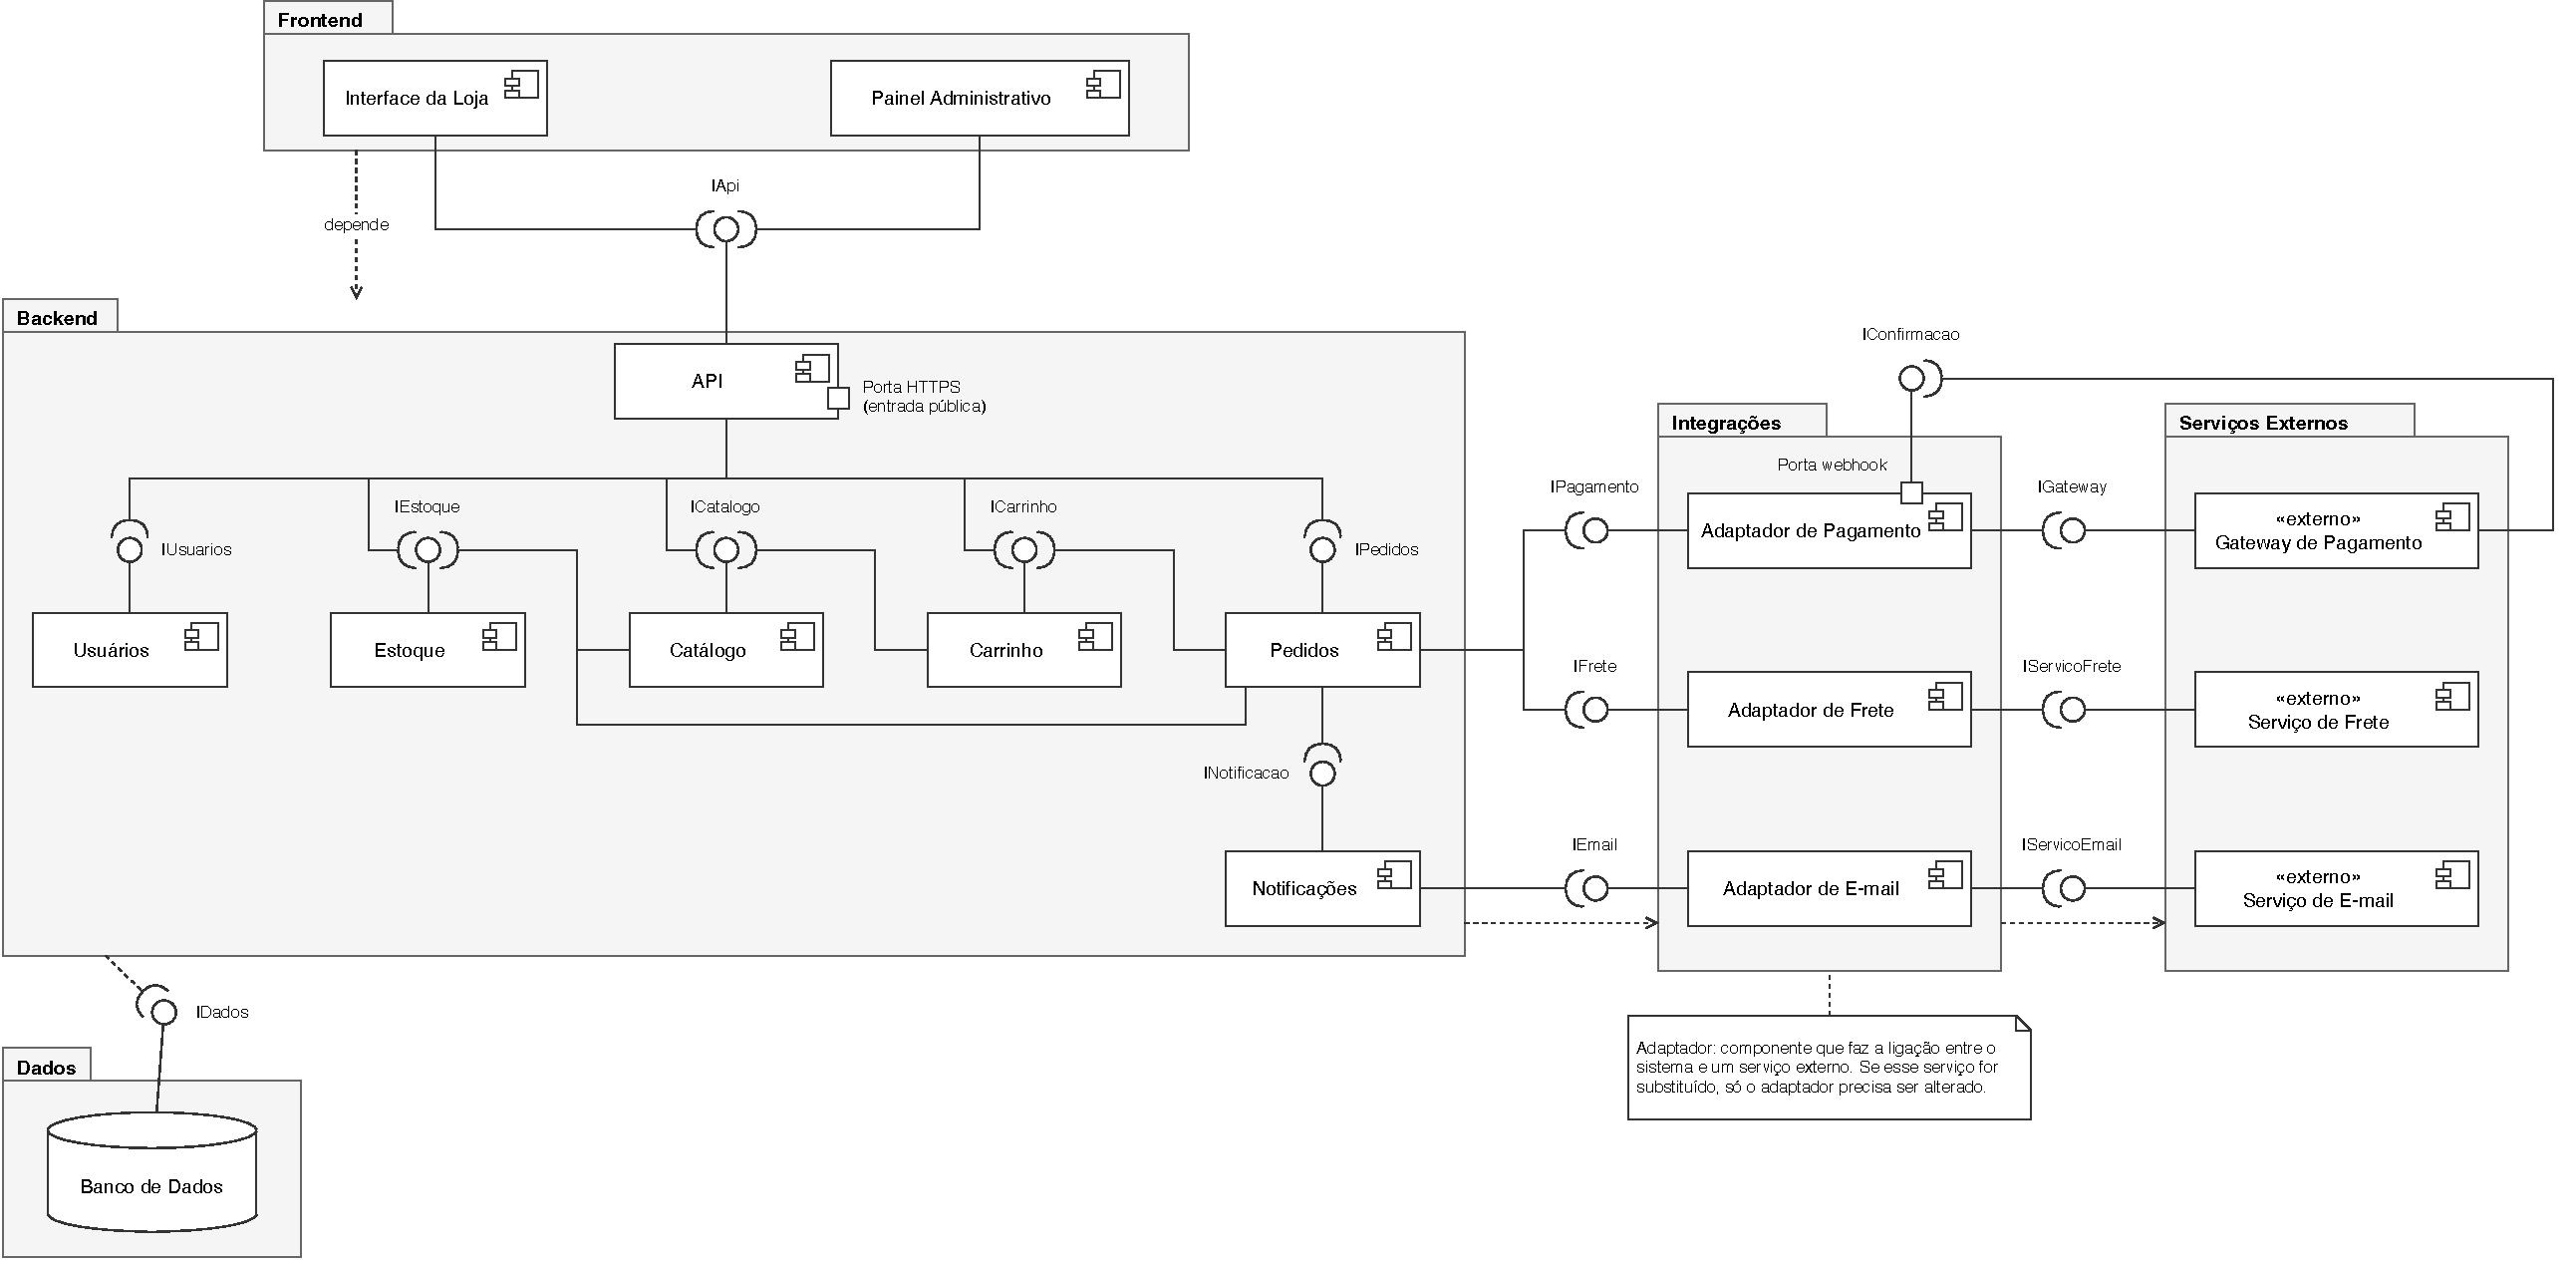
\includegraphics[width=0.9\textwidth,keepaspectratio]{../assets/CMP_Geral.pdf}
\caption{Diagrama de Componentes: visão geral}
\fonte{elaborado pelos autores no draw.io (2026).}
\end{figure}

\subsection{Dicionário de Componentes}

{\small
{\arrayrulecolor{ghlight}\setlength{\arrayrulewidth}{0.3pt}\renewcommand{\arraystretch}{1.15}\rowcolors{2}{ghbg}{white}
\begin{xltabular}{\textwidth}{>{\raggedright\arraybackslash}p{2.7cm}|>{\raggedright\arraybackslash}X|>{\raggedright\arraybackslash}p{2.6cm}|>{\raggedright\arraybackslash}p{3.0cm}}
\rowcolor{white}\caption{Dicionário de componentes (visão geral)}\label{tab:dicionario}\\
\arrayrulecolor{black}\toprule\arrayrulecolor{ghlight}
\rowcolor{ghbg}\textbf{Componente} & \textbf{Responsabilidade} & \textbf{Fornece} & \textbf{Requer}\\ \arrayrulecolor{black}\midrule\arrayrulecolor{ghlight}
\endfirsthead
\arrayrulecolor{black}\toprule\arrayrulecolor{ghlight}
\rowcolor{ghbg}\textbf{Componente} & \textbf{Responsabilidade} & \textbf{Fornece} & \textbf{Requer}\\ \arrayrulecolor{black}\midrule\arrayrulecolor{ghlight}
\endhead
\endlastfoot
Interface da Loja & Telas de catálogo, carrinho, finalização do pedido e pedidos. & Nenhuma & \texttt{IApi}\\ \hline
Painel Administrativo & Telas de produtos, estoque e pedidos. & Nenhuma & \texttt{IApi}\\ \hline
API & Entrada HTTPS; valida sessão e perfil; encaminha às funções dos módulos. No detalhe do Backend, corresponde à camada de API (controladores e segurança). & \texttt{IApi} & \texttt{IUsuarios}, \texttt{ICatalogo}, \texttt{ICarrinho}, \texttt{IPedidos}, \texttt{IEstoque}\\ \hline
Usuários & Cadastro, login e perfis. & \texttt{IUsuarios} & \texttt{IDados} (via Repositórios)\\ \hline
Catálogo & Produtos, categorias, marcas, filtros e busca. & \texttt{ICatalogo} & \texttt{IDados} (via Repositórios), \texttt{IEstoque}\\ \hline
Carrinho & Itens e subtotal. & \texttt{ICarrinho} & \texttt{ICatalogo}\\ \hline
Pedidos & Finalização do pedido, status e cancelamento. & \texttt{IPedidos} & \texttt{ICarrinho}, \texttt{IEstoque}, \texttt{IFrete}, \texttt{IPagamento}, \texttt{INotificacao}, \texttt{IDados} (via Repositórios)\\ \hline
Estoque & Disponibilidade, reserva, baixa e ajustes. & \texttt{IEstoque} & \texttt{IDados} (via Repositórios)\\ \hline
Notificações & Monta e envia e-mails de status. & \texttt{INotificacao} & \texttt{IEmail}\\ \hline
Adaptador de Pagamento & Comunica-se com o gateway de pagamento. & \texttt{IPagamento} & \texttt{IGateway}\\ \hline
Adaptador de Frete & Comunica-se com o serviço de frete. & \texttt{IFrete} & \texttt{IServicoFrete}\\ \hline
Adaptador de E-mail & Comunica-se com o serviço de e-mail. & \texttt{IEmail} & \texttt{IServicoEmail}\\ \hline
Banco de Dados & Persistência dos dados. & \texttt{IDados} & Nenhuma\\ \hline
Gateway de Pagamento, Serviço de Frete, Serviço de E-mail (externos) & Serviços de terceiros. & \texttt{IGateway}, \texttt{IServicoFrete}, \texttt{IServicoEmail} & Nenhuma\\ \arrayrulecolor{black}\bottomrule
\end{xltabular}}
}

\paragraph{Interfaces do sistema.} O quadro abaixo explica o que cada interface representa. O nome começa com a letra I (de \emph{interface}).

{\arrayrulecolor{ghlight}\setlength{\arrayrulewidth}{0.3pt}\renewcommand{\arraystretch}{1.15}\rowcolors{2}{ghbg}{white}
\begin{xltabular}{\textwidth}{>{\raggedright\arraybackslash}p{3.6cm}|>{\raggedright\arraybackslash}X}
\rowcolor{white}\caption{Interfaces do sistema}\\
\arrayrulecolor{black}\toprule\arrayrulecolor{ghlight}
\rowcolor{ghbg}\textbf{Interface} & \textbf{O que oferece}\\ \arrayrulecolor{black}\midrule\arrayrulecolor{ghlight}
\endfirsthead
\arrayrulecolor{black}\toprule\arrayrulecolor{ghlight}
\rowcolor{ghbg}\textbf{Interface} & \textbf{O que oferece}\\ \arrayrulecolor{black}\midrule\arrayrulecolor{ghlight}
\endhead
\endlastfoot
\texttt{IApi} & Recebe as solicitações das telas. Oferecida pela API.\\ \hline
\texttt{IUsuarios} & Cadastro, login e perfis de usuário.\\ \hline
\texttt{ICatalogo} & Consulta de produtos, categorias e marcas, com filtros e busca.\\ \hline
\texttt{ICarrinho} & Gerenciamento dos itens e do subtotal do carrinho.\\ \hline
\texttt{IPedidos} & Criação de pedidos, acompanhamento do status e cancelamento.\\ \hline
\texttt{IEstoque} & Consulta de disponibilidade, reserva, baixa e ajuste das quantidades.\\ \hline
\texttt{INotificacao} & Envio de avisos ao cliente sobre o pedido.\\ \hline
\texttt{IPagamento} & Cobrança e estorno de pagamentos. Oferecida pelo adaptador de pagamento.\\ \hline
\texttt{IFrete} & Cálculo de valor e prazo de entrega. Oferecida pelo adaptador de frete.\\ \hline
\texttt{IEmail} & Envio de e-mails. Oferecida pelo adaptador de e-mail.\\ \hline
\texttt{IDados} & Gravação e consulta de dados no banco de dados.\\ \hline
\texttt{IGateway}, \texttt{IServicoFrete}, \texttt{IServicoEmail} & Serviços oferecidos pelos sistemas externos: cobrança e estorno, cotação de frete e envio de e-mail.\\ \arrayrulecolor{black}\bottomrule
\end{xltabular}}

\paragraph{Leitura do diagrama.} As setas tracejadas entre os pacotes indicam dependência: o Frontend depende do Backend, o Backend depende das Integrações e as Integrações dependem dos Serviços Externos. Os módulos usam o banco de dados por meio dos Repositórios (descritos na seção \ref{sec:backend-detalhe}); por isso a dependência de \texttt{IDados} aparece no nível do pacote Backend, e não em cada módulo.

\paragraph{Justificativa das dependências.} A \emph{API} é o único ponto
de entrada, o que centraliza segurança e controle de perfil. \emph{Pedidos}
depende de \emph{Carrinho}, \emph{Estoque}, \emph{Frete}, \emph{Pagamento}
e \emph{Notificações} porque a finalização do pedido orquestra esses serviços. O
\emph{Catálogo} consulta \emph{Estoque} para exibir a disponibilidade, e o
\emph{Carrinho} obtém preço e disponibilidade pelo \emph{Catálogo}.
Nenhum módulo de negócio acessa serviço externo diretamente, apenas
pelos adaptadores. Há duas \textbf{portas}: a porta HTTPS da \emph{API}
(entrada pública) e a porta de \emph{webhook} do \emph{Adaptador de
Pagamento} (confirmação de Pix e boleto).

\subsection{Detalhe Interno: Frontend}

O \emph{Frontend} reúne as duas aplicações de interface. Cada uma é
dividida em telas (componentes internos) que compartilham o componente
\emph{Cliente da API}, responsável pela sessão e pelas requisições
HTTPS. Esse é o único ponto do Frontend que requer a interface
\texttt{IApi}.

\begin{figure}[H]
\centering
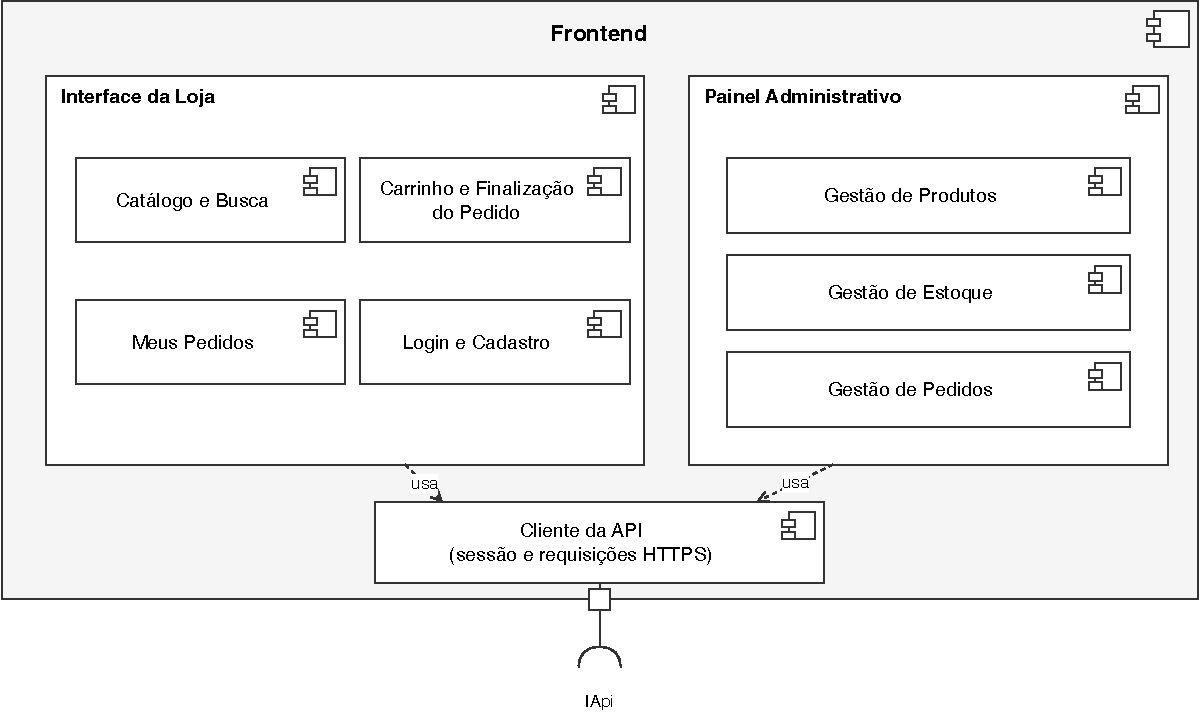
\includegraphics[width=\textwidth,height=0.45\textheight,keepaspectratio]{../assets/CMP_Frontend.pdf}
\caption{Diagrama de Componentes: detalhe do Frontend}
\fonte{elaborado pelos autores no draw.io (2026).}
\end{figure}

{\arrayrulecolor{ghlight}\setlength{\arrayrulewidth}{0.3pt}\renewcommand{\arraystretch}{1.15}\rowcolors{2}{ghbg}{white}
\begin{xltabular}{\textwidth}{>{\raggedright\arraybackslash}p{4.6cm}|>{\raggedright\arraybackslash}X}
\rowcolor{white}\caption{Componentes internos do Frontend}\\
\arrayrulecolor{black}\toprule\arrayrulecolor{ghlight}
\rowcolor{ghbg}\textbf{Componente interno} & \textbf{Responsabilidade}\\ \arrayrulecolor{black}\midrule\arrayrulecolor{ghlight}
\endfirsthead
\arrayrulecolor{black}\toprule\arrayrulecolor{ghlight}
\rowcolor{ghbg}\textbf{Componente interno} & \textbf{Responsabilidade}\\ \arrayrulecolor{black}\midrule\arrayrulecolor{ghlight}
\endhead
\endlastfoot
Catálogo e Busca & Listagem, filtros, busca e detalhes dos produtos (CU\nobreakdash-01).\\ \hline
Carrinho e Finalização do Pedido & Carrinho, escolha de frete e pagamento e confirmação do pedido (CU\nobreakdash-02 e CU\nobreakdash-03).\\ \hline
Meus Pedidos & Consulta e cancelamento de pedidos (CU\nobreakdash-04 e CU\nobreakdash-08).\\ \hline
Login e Cadastro & Cadastro de cliente e autenticação (CU\nobreakdash-09 e CU\nobreakdash-12).\\ \hline
Gestão de Produtos & Cadastro, edição e inativação de produtos (CU\nobreakdash-05).\\ \hline
Gestão de Estoque & Ajuste de quantidades em estoque (CU\nobreakdash-05).\\ \hline
Gestão de Pedidos & Consulta de pedidos e atualização de status (CU\nobreakdash-06, que dispara o CU\nobreakdash-13).\\ \hline
Cliente da API & Mantém a sessão e envia as requisições HTTPS; requer \texttt{IApi}.\\ \arrayrulecolor{black}\bottomrule
\end{xltabular}}

\subsection{Detalhe Interno: Backend}\label{sec:backend-detalhe}

O \emph{Backend} é organizado em três pacotes (camadas): a \textbf{camada
de API} (controladores e segurança), os \textbf{módulos de negócio} e o
\textbf{acesso a dados}. As setas tracejadas indicam que a camada de API usa
as interfaces dos módulos e que os módulos usam o acesso a dados. Cada
módulo oferece a sua própria interface (círculo). A camada de API corresponde ao componente API do diagrama geral e fornece
\texttt{IApi} pelas portas no topo, uma para cada controlador; \emph{Pedidos} requer \texttt{IPagamento}
e \texttt{IFrete}, \emph{Notificações} requer \texttt{IEmail} e os
\emph{Repositórios} requerem \texttt{IDados}, todos por portas na base. As
dependências entre os módulos (por exemplo, Pedidos usando Carrinho) já
aparecem no diagrama geral e não são repetidas aqui.

\begin{figure}[H]
\centering
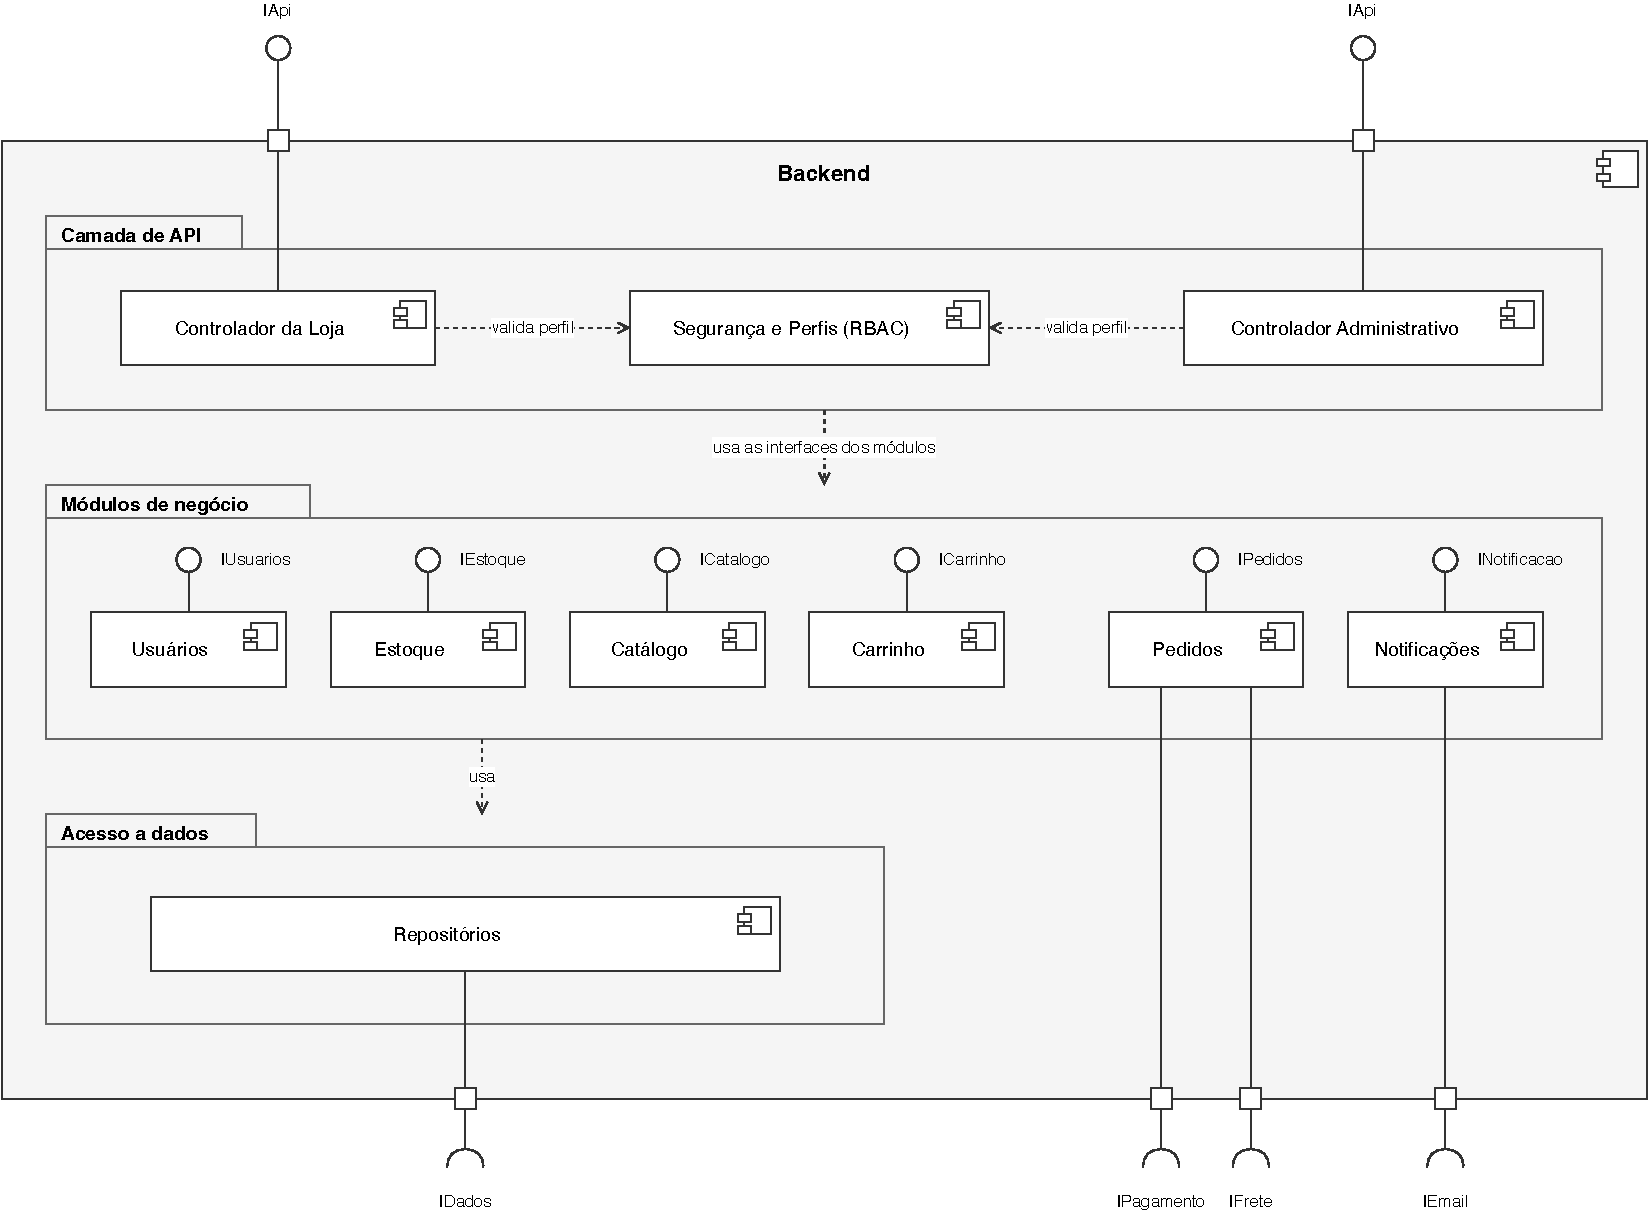
\includegraphics[width=\textwidth,height=0.5\textheight,keepaspectratio]{../assets/CMP_Backend.pdf}
\caption{Diagrama de Componentes: detalhe do Backend}
\fonte{elaborado pelos autores no draw.io (2026).}
\end{figure}

{\arrayrulecolor{ghlight}\setlength{\arrayrulewidth}{0.3pt}\renewcommand{\arraystretch}{1.15}\rowcolors{2}{ghbg}{white}
\begin{xltabular}{\textwidth}{>{\raggedright\arraybackslash}p{4.6cm}|>{\raggedright\arraybackslash}X}
\rowcolor{white}\caption{Componentes internos do Backend}\\
\arrayrulecolor{black}\toprule\arrayrulecolor{ghlight}
\rowcolor{ghbg}\textbf{Componente interno} & \textbf{Responsabilidade}\\ \arrayrulecolor{black}\midrule\arrayrulecolor{ghlight}
\endfirsthead
\arrayrulecolor{black}\toprule\arrayrulecolor{ghlight}
\rowcolor{ghbg}\textbf{Componente interno} & \textbf{Responsabilidade}\\ \arrayrulecolor{black}\midrule\arrayrulecolor{ghlight}
\endhead
\endlastfoot
Controlador da Loja & Recebe as requisições do cliente e do visitante; fornece \texttt{IApi}.\\ \hline
Controlador Administrativo & Recebe as requisições do administrador; fornece \texttt{IApi}.\\ \hline
Segurança e Perfis (RBAC) & Valida a sessão e o perfil antes de cada operação; é usado pelos dois controladores.\\ \hline
Usuários, Catálogo, Estoque, Carrinho, Pedidos, Notificações & Módulos de negócio descritos no Quadro~\ref{tab:dicionario}.\\ \hline
Repositórios & Gravam e consultam os dados dos módulos; requerem \texttt{IDados}.\\ \arrayrulecolor{black}\bottomrule
\end{xltabular}}

% =========================================================================
\section{Ferramenta de Modelagem e Lista de Símbolos}\label{sec:simbolos}

Os diagramas foram elaborados no \textbf{draw.io} (diagrams.net).

{\arrayrulecolor{ghlight}\setlength{\arrayrulewidth}{0.3pt}\renewcommand{\arraystretch}{1.0}\small\rowcolors{2}{ghbg}{white}
\begin{xltabular}{\textwidth}{>{\raggedright\arraybackslash}p{4.2cm}|>{\raggedright\arraybackslash}p{5.6cm}|>{\raggedright\arraybackslash}X}
\rowcolor{white}\caption{Símbolos do diagrama de casos de uso (ferramenta: draw.io)}\\
\arrayrulecolor{black}\toprule\arrayrulecolor{ghlight}
\rowcolor{ghbg}\textbf{Elemento} & \textbf{Símbolo no draw.io} & \textbf{Significado}\\ \arrayrulecolor{black}\midrule\arrayrulecolor{ghlight}
\endfirsthead
\arrayrulecolor{black}\toprule\arrayrulecolor{ghlight}
\rowcolor{ghbg}\textbf{Elemento} & \textbf{Símbolo no draw.io} & \textbf{Significado}\\ \arrayrulecolor{black}\midrule\arrayrulecolor{ghlight}
\endhead
\endlastfoot
Ator principal & Boneco com o nome abaixo & Usuário que usa o sistema diretamente.\\ \hline
Ator secundário & Boneco com o nome e o estereótipo \texttt{<<sistema>>} & Sistema externo com o qual o sistema se comunica (gateway, frete, e-mail).\\ \hline
Caso de uso & Elipse com o nome dentro & Funcionalidade oferecida ao ator.\\ \hline
Fronteira do sistema & Retângulo com o nome do sistema no topo & Delimita o escopo modelado.\\ \hline
Associação & Linha contínua & Comunicação entre ator e caso de uso.\\ \hline
Generalização & Linha com ponta de triângulo vazada & Herança entre atores (Cliente $\to$ Visitante).\\ \hline
\texttt{<<include>>} & Seta tracejada com estereótipo & Passo obrigatório incluído em outro caso de uso.\\ \hline
\texttt{<<extend>>} & Seta tracejada com estereótipo, ligada por linha tracejada a uma nota com a condição & Fluxo opcional que estende outro caso de uso, só quando a condição é verdadeira.\\ \arrayrulecolor{black}\bottomrule
\end{xltabular}}

{\arrayrulecolor{ghlight}\setlength{\arrayrulewidth}{0.3pt}\renewcommand{\arraystretch}{1.0}\small\rowcolors{2}{ghbg}{white}
\begin{xltabular}{\textwidth}{>{\raggedright\arraybackslash}p{4.2cm}|>{\raggedright\arraybackslash}p{5.6cm}|>{\raggedright\arraybackslash}X}
\rowcolor{white}\caption{Símbolos do diagrama de componentes (ferramenta: draw.io)}\\
\arrayrulecolor{black}\toprule\arrayrulecolor{ghlight}
\rowcolor{ghbg}\textbf{Elemento} & \textbf{Símbolo no draw.io} & \textbf{Significado}\\ \arrayrulecolor{black}\midrule\arrayrulecolor{ghlight}
\endfirsthead
\arrayrulecolor{black}\toprule\arrayrulecolor{ghlight}
\rowcolor{ghbg}\textbf{Elemento} & \textbf{Símbolo no draw.io} & \textbf{Significado}\\ \arrayrulecolor{black}\midrule\arrayrulecolor{ghlight}
\endhead
\endlastfoot
Componente & Retângulo com o ícone de componente no canto superior direito & Módulo lógico do sistema.\\ \hline
Pacote & Retângulo em forma de pasta, com o nome na aba & Agrupa componentes (Frontend, Backend\ldots).\\ \hline
Interface fornecida & Círculo (``pirulito'') ligado ao componente & Serviço que o componente oferece.\\ \hline
Interface requerida & Meio-círculo (``soquete'') voltado ao círculo & Serviço de que o componente precisa.\\ \hline
Dependência & Seta tracejada aberta & Um elemento depende de outro.\\ \hline
Porta & Pequeno quadrado na borda do componente & Ponto de interação do componente com o ambiente externo.\\ \hline
Banco de dados & Cilindro & Local onde os dados são guardados.\\ \arrayrulecolor{black}\bottomrule
\end{xltabular}}


% =========================================================================
\section*{REFERÊNCIAS}
\addcontentsline{toc}{section}{REFERÊNCIAS}

\begin{singlespace}
\noindent OBJECT MANAGEMENT GROUP (OMG). \textbf{Unified Modeling
Language (UML) Specification}, versão 2.5.1. Disponível em:
\url{https://www.omg.org/spec/UML/2.5.1}.

\vspace{0.3cm}
\noindent JGRAPH LTD. \textbf{draw.io (diagrams.net)}. Disponível em:
\url{https://app.diagrams.net}.

\vspace{0.3cm}
\noindent ASSOCIAÇÃO BRASILEIRA DE NORMAS TÉCNICAS. \textbf{NBR 14724:
Informação e documentação: trabalhos acadêmicos: apresentação}.
Rio de Janeiro: ABNT, 2011.
\end{singlespace}

% =========================================================================
\newpage
\appendix
\titleformat{\section}
  {\normalfont\normalsize\bfseries\MakeUppercase}{APÊNDICE \Alph{section}:}{0.5em}{}
\section{Requisitos e Regras de Negócio}\label{sec:apendice}

\Needspace{10\baselineskip}
\subsection*{Requisitos Funcionais}

{\arrayrulecolor{ghlight}\setlength{\arrayrulewidth}{0.3pt}\renewcommand{\arraystretch}{1.15}\rowcolors{2}{ghbg}{white}
\begin{xltabular}{\textwidth}{>{\raggedright\arraybackslash}p{1.6cm}|>{\raggedright\arraybackslash}X}
\rowcolor{white}\caption{Requisitos funcionais}\\
\arrayrulecolor{black}\toprule\arrayrulecolor{ghlight}
\rowcolor{ghbg}\textbf{ID} & \textbf{Requisito}\\ \arrayrulecolor{black}\midrule\arrayrulecolor{ghlight}
\endfirsthead
\arrayrulecolor{black}\toprule\arrayrulecolor{ghlight}
\rowcolor{ghbg}\textbf{ID} & \textbf{Requisito}\\ \arrayrulecolor{black}\midrule\arrayrulecolor{ghlight}
\endhead
\endlastfoot
RF-01 & Listar produtos do catálogo com filtros por categoria, marca e faixa de preço, além de busca por texto.\\ \hline
RF-02 & Exibir detalhes do produto (descrição, preço, disponibilidade).\\ \hline
RF-03 & Cadastrar e autenticar cliente (e-mail e senha).\\ \hline
RF-04 & Adicionar, alterar e remover itens do carrinho.\\ \hline
RF-05 & Calcular frete por CEP via serviço externo.\\ \hline
RF-06 & Finalizar pedido (endereço, frete, forma de pagamento, confirmação).\\ \hline
RF-07 & Processar pagamento pelo gateway de pagamento (cartão, Pix ou boleto).\\ \hline
RF-08 & Consultar os pedidos e o status deles e cancelar antes do envio (com estorno se já pago).\\ \hline
RF-09 & Avisar o cliente por e-mail nas mudanças de status do pedido, inclusive no cancelamento.\\ \hline
RF-10 & Cadastrar, editar e inativar produtos (administrador).\\ \hline
RF-11 & Gerenciar estoque: ajustar quantidades (administrador).\\ \hline
RF-12 & Consultar pedidos e atualizar o status (administrador).\\ \arrayrulecolor{black}\bottomrule
\end{xltabular}}

\Needspace{10\baselineskip}
\subsection*{Requisitos Não Funcionais}

{\arrayrulecolor{ghlight}\setlength{\arrayrulewidth}{0.3pt}\renewcommand{\arraystretch}{1.15}\rowcolors{2}{ghbg}{white}
\begin{xltabular}{\textwidth}{>{\raggedright\arraybackslash}p{1.6cm}|>{\raggedright\arraybackslash}X}
\rowcolor{white}\caption{Requisitos não funcionais}\\
\arrayrulecolor{black}\toprule\arrayrulecolor{ghlight}
\rowcolor{ghbg}\textbf{ID} & \textbf{Requisito}\\ \arrayrulecolor{black}\midrule\arrayrulecolor{ghlight}
\endfirsthead
\arrayrulecolor{black}\toprule\arrayrulecolor{ghlight}
\rowcolor{ghbg}\textbf{ID} & \textbf{Requisito}\\ \arrayrulecolor{black}\midrule\arrayrulecolor{ghlight}
\endhead
\endlastfoot
RNF-01 & Comunicação por HTTPS; senhas com hash.\\ \hline
RNF-02 & Acesso por perfil: área administrativa restrita ao Administrador.\\ \hline
RNF-03 & Dados de cartão não são armazenados pela loja (tratados pelo gateway de pagamento).\\ \hline
RNF-04 & Interface responsiva (celular e desktop).\\ \hline
RNF-05 & Falha em serviço externo não derruba o restante do sistema.\\ \hline
RNF-06 & Arquitetura modular, com interfaces bem definidas, para trocar o gateway de pagamento ou o serviço de frete sem afetar o núcleo.\\ \arrayrulecolor{black}\bottomrule
\end{xltabular}}

\Needspace{10\baselineskip}
\subsection*{Regras de Negócio}

{\arrayrulecolor{ghlight}\setlength{\arrayrulewidth}{0.3pt}\renewcommand{\arraystretch}{1.15}\rowcolors{2}{ghbg}{white}
\begin{xltabular}{\textwidth}{>{\raggedright\arraybackslash}p{1.6cm}|>{\raggedright\arraybackslash}X}
\rowcolor{white}\caption{Regras de negócio}\\
\arrayrulecolor{black}\toprule\arrayrulecolor{ghlight}
\rowcolor{ghbg}\textbf{ID} & \textbf{Regra}\\ \arrayrulecolor{black}\midrule\arrayrulecolor{ghlight}
\endfirsthead
\arrayrulecolor{black}\toprule\arrayrulecolor{ghlight}
\rowcolor{ghbg}\textbf{ID} & \textbf{Regra}\\ \arrayrulecolor{black}\midrule\arrayrulecolor{ghlight}
\endhead
\endlastfoot
RN-01 & Só produtos ativos aparecem no catálogo; sem estoque, o produto fica indisponível.\\ \hline
RN-02 & A quantidade no carrinho não pode exceder o estoque disponível.\\ \hline
RN-03 & Só cliente autenticado finaliza pedido.\\ \hline
RN-04 & O estoque é reservado ao criar o pedido e baixado quando o pagamento é aprovado.\\ \hline
RN-05 & O pedido pode ser cancelado até o envio; se já estava pago, o valor é estornado.\\ \hline
RN-06 & Falha ao enviar e-mail não desfaz nenhuma operação.\\ \arrayrulecolor{black}\bottomrule
\end{xltabular}}

\noindent\textbf{Status do pedido:} aguardando pagamento $\rightarrow$ pago $\rightarrow$ em separação $\rightarrow$ enviado $\rightarrow$ entregue. O pedido pode ser cancelado a partir de qualquer status anterior a enviado.

\section{Glossário de Termos Técnicos}\label{sec:termos}

O quadro a seguir explica, em linguagem simples, os termos técnicos usados ao longo do documento.

{\arrayrulecolor{ghlight}\setlength{\arrayrulewidth}{0.3pt}\renewcommand{\arraystretch}{1.0}\small\rowcolors{2}{ghbg}{white}
\begin{xltabular}{\textwidth}{>{\raggedright\arraybackslash}p{3.6cm}|>{\raggedright\arraybackslash}X}
\rowcolor{white}\caption{Termos técnicos utilizados}\\
\arrayrulecolor{black}\toprule\arrayrulecolor{ghlight}
\rowcolor{ghbg}\textbf{Termo} & \textbf{O que significa}\\ \arrayrulecolor{black}\midrule\arrayrulecolor{ghlight}
\endfirsthead
\arrayrulecolor{black}\toprule\arrayrulecolor{ghlight}
\rowcolor{ghbg}\textbf{Termo} & \textbf{O que significa}\\ \arrayrulecolor{black}\midrule\arrayrulecolor{ghlight}
\endhead
\endlastfoot
Gateway de pagamento & Serviço externo que recebe os dados da compra, cobra o cliente (cartão, Pix ou boleto) e informa se o pagamento foi aprovado.\\ \hline
Webhook & Aviso automático que o gateway de pagamento envia ao sistema quando um pagamento é confirmado. É usado no Pix e no boleto, que não são aprovados na hora.\\ \hline
RBAC (controle de acesso por perfil) & Regra que define o que cada tipo de usuário pode fazer. Por exemplo, só o administrador acessa a área de produtos e estoque.\\ \hline
HTTPS & Forma segura de comunicação pela internet, que protege os dados trocados, como senhas e endereços.\\ \hline
Frontend & Parte do sistema que o usuário vê e usa, ou seja, as telas.\\ \hline
Backend & Parte interna do sistema, que executa as regras do negócio e guarda os dados.\\ \hline
API & Ponto de entrada do backend. Recebe as solicitações das telas e as encaminha ao módulo responsável.\\ \hline
Adaptador & Componente que faz a ``tradução'' entre o sistema e um serviço externo. Assim, o serviço pode ser trocado sem alterar o resto do sistema.\\ \hline
Controlador & Componente da API que recebe as solicitações de um tipo de usuário (cliente ou administrador) e as repassa aos módulos.\\ \hline
Repositório & Componente que grava e consulta os dados no banco de dados.\\ \hline
Cliente da API & Componente do frontend que envia as solicitações das telas à API e mantém a sessão do usuário (o login ativo).\\ \hline
Interface & Conjunto de serviços de um componente. A \emph{fornecida} (círculo) é o que ele oferece; a \emph{requerida} (meio-círculo) é o que ele precisa de outro componente.\\ \hline
Porta & Ponto de entrada ou saída de um componente, por onde ele se comunica com o ambiente externo.\\ \arrayrulecolor{black}\bottomrule
\end{xltabular}}

\end{document}
